\chapter{Simuleren van gedrag op basis van een sequentiediagram}\label{sec:gedrag}
Een ander populair type van UML-diagram is het sequentiediagram. Waar klassediagrammen de informatie bevat in klasses en de verbanden tussen klasses benoemen, beschrijven sequentiediagrammen het gedrag van instanties van de klasses. Deze instanties communiceren via berichten. Doorgaans zijn deze berichten ofwel een oproep van een methode gedefinieerd voor de klasse van een instantie ofwel een instantiatie van een nieuwe instantie. De berichten zijn genummerd volgens een bepaalde volgorde en samen modelleren ze het gedrag van een stuk van de software.

\parbreak

Figuur \ref{fig:seq-diagram-game} geeft een voorbeeld van een sequentiediagram gebaseerd op het klassediagram voorgesteld in figuur \ref{fig:diagram-voorbeeld}.

Een instantie wordt voorgesteld door een kader met daarin tekst volgens het patroon \textit{instantienaam : klassenaam}. Dit wil zeggen dat bijvoorbeeld \textit{attacker} een instantie is van de klasse \textit{Character}. Vanuit elk kader vertrekt ook een streepjeslijn: de \textbf{levenslijn}. Deze levenslijn kan ingevuld worden door gekleurde balken, welke de duur van een oproep van een methode aan een instantie voorstellen.
Verder zijn er ook kaders die berichten omsluiten. Deze kaders duiden \textbf{gecombineerde fragmenten} aan, en in deze tekst beschouwen we twee soorten:

\begin{enumerate}
	\item Het \textbf{altfragment}: Deze soort duidt een \textit{if-else}-constructie aan. Het bestaat uit twee delen, namelijk het \text{if}-deel en het \textit{else}-deel, en er staat aangeduid onder welke voorwaarden welk deel wordt uitgevoerd. Figuur \ref{fig:seq-diagram-game} bevat een voorbeeld van een altfragment.
	\item Het \textbf{lusfragment}: Deze soort duidt een lusconstructie aan. Er staat aangeduid onder welke voorwaarden er een iteratie wordt uitgevoerd. Deze voorwaarde wordt gecontroleerd zowel v\'o\'or de eerste keer dat er mogelijks een iteratie wordt uitgevoerd als elke keer dat een iteratie ten einde komt. Indien de voorwaarde niet geldt, wordt de lus overgeslagen. \todo{referentie naar figuur met loop fragment}
\end{enumerate}

In dit hoofdstuk beschouwen we hoe we het vocabularium en de logische theorie die we hebben opgebouwd eerder in de tekst kunnen uitbreiden om het gedrag voorgesteld in een sequentiediagram te modelleren.

\begin{landscape}
\begin{figure}
	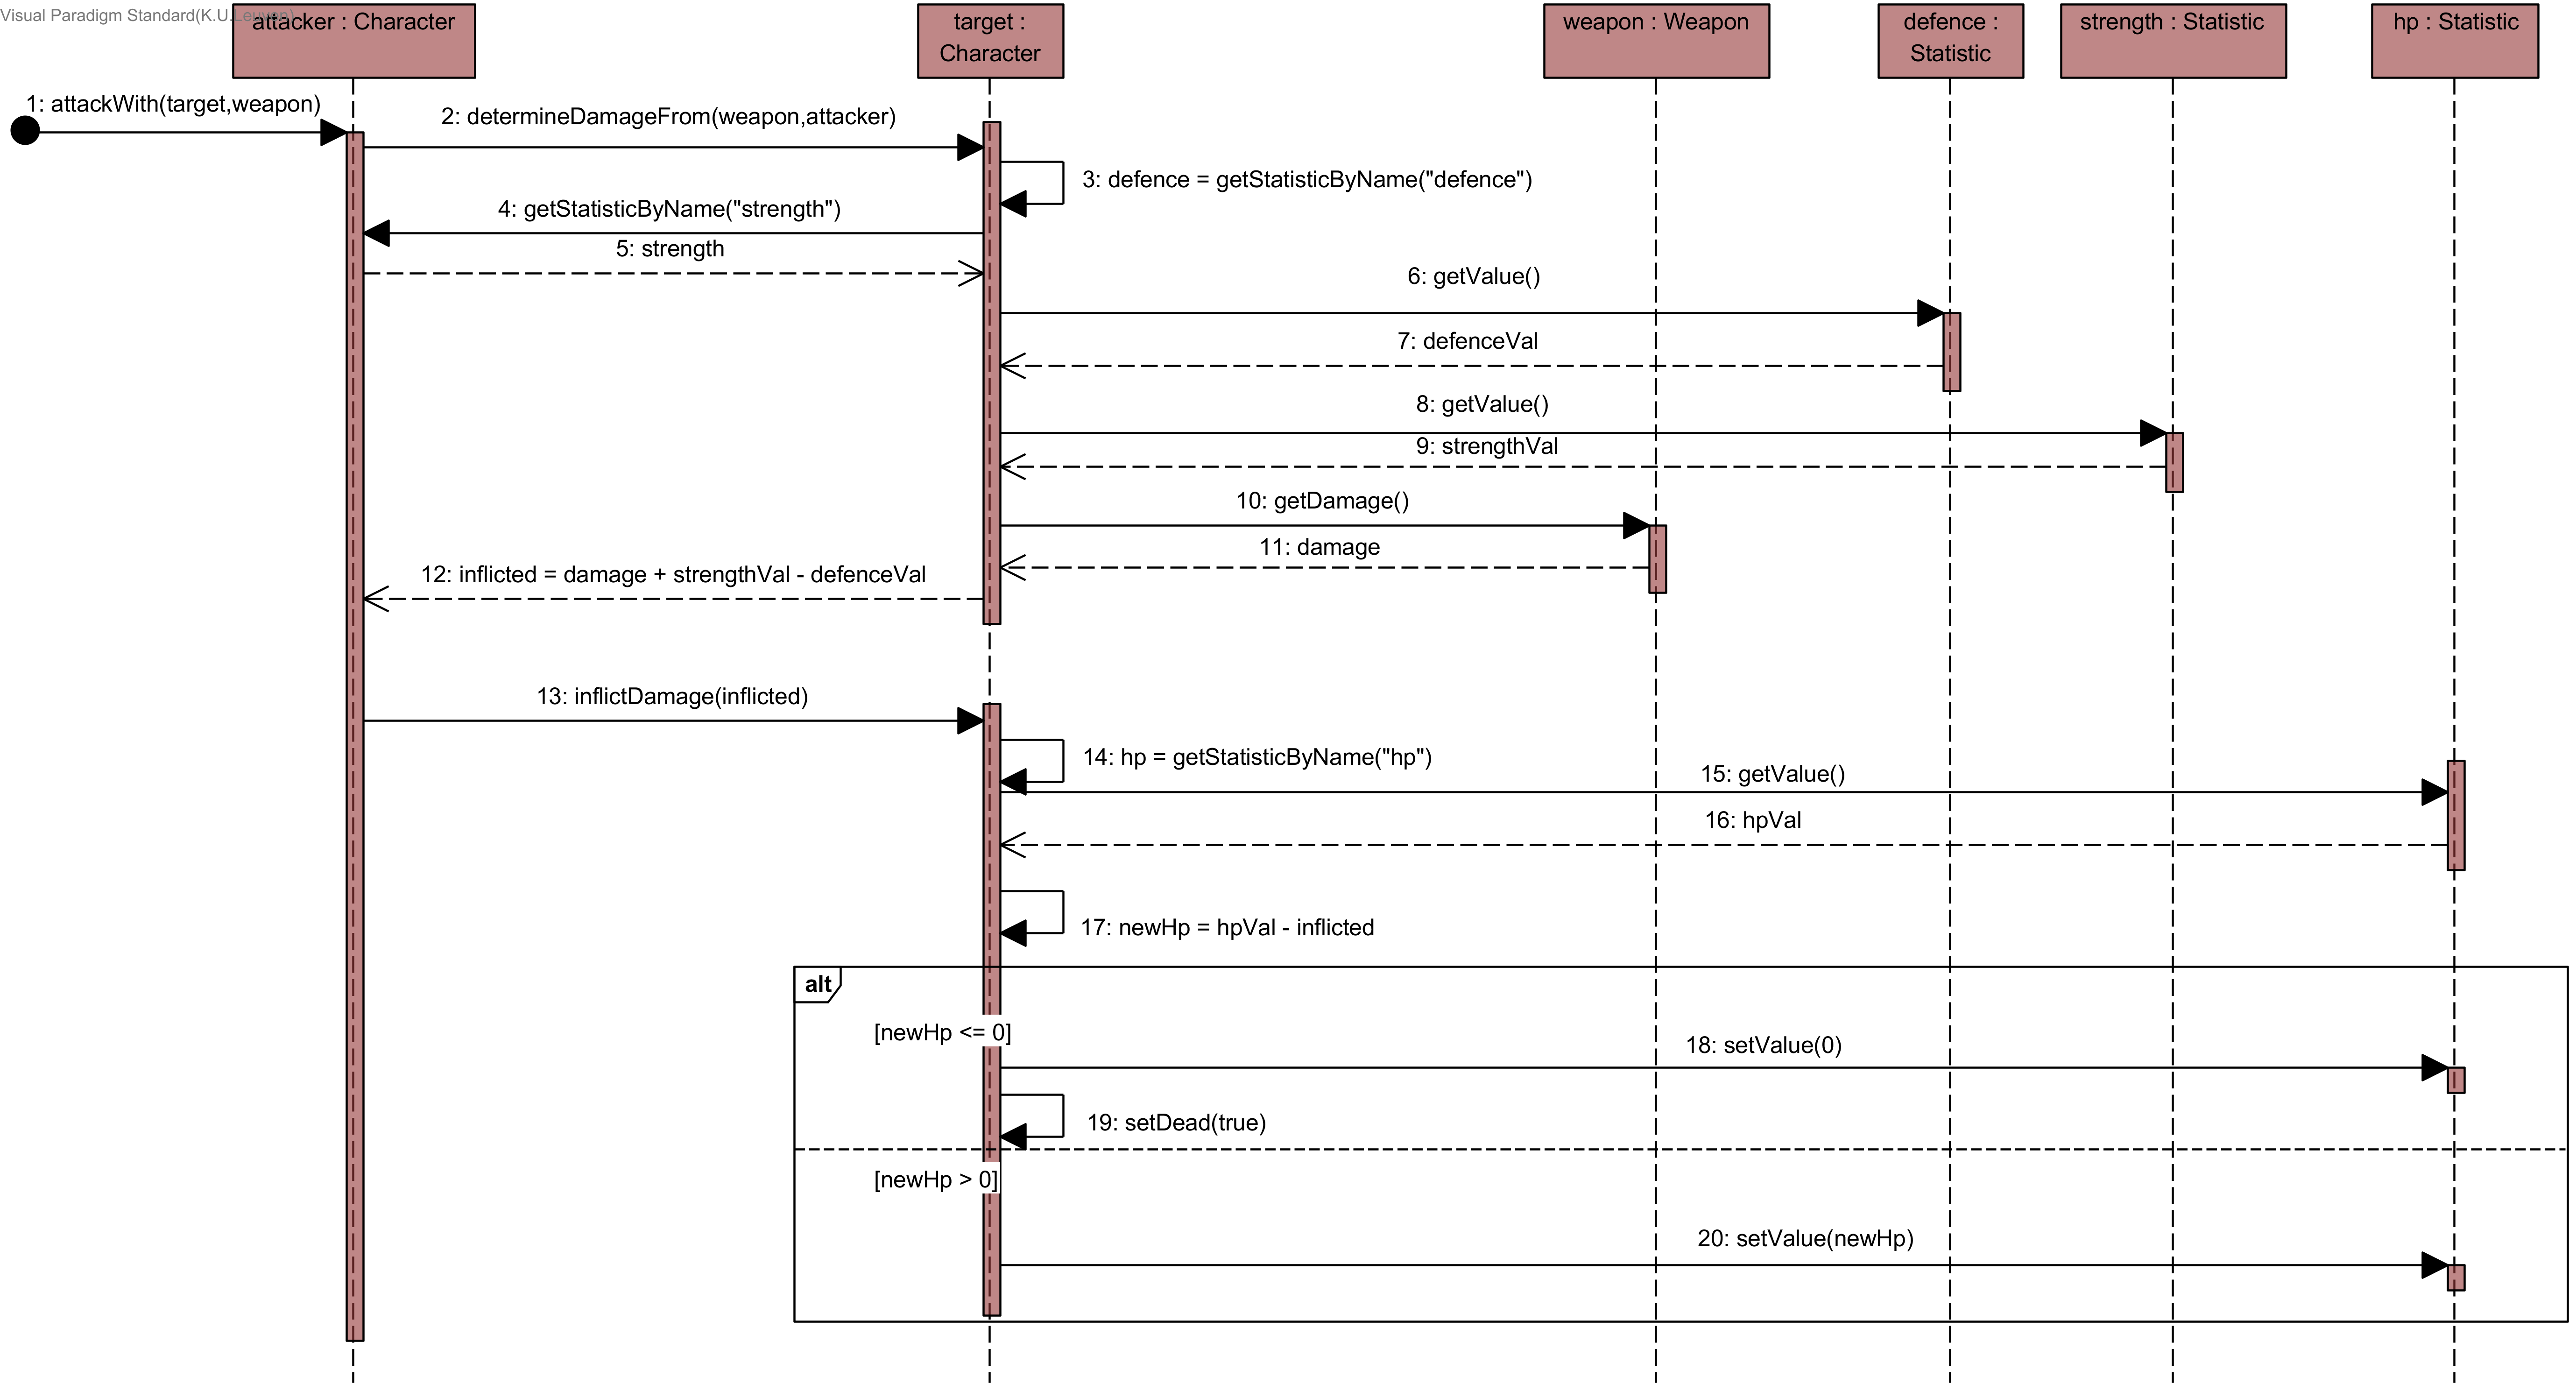
\includegraphics[width=1.5\textwidth]{chap-gedrag/seq-diagram-game.png}
	\caption{Sequentiediagram gebaseerd op het klassediagram van figuur \ref{fig:diagram-voorbeeld}}
	\label{fig:seq-diagram-game}
\end{figure}
\end{landscape}

\section{De keuze voor lineaire tijdscalculus}
UML-diagrammen schrijven mogelijke toestanden van, en acties, op softwaresystemen voor. Die systemen kunnen van toestand veranderen tussen tijdstappen. Sequentiediagrammen zijn een manier om te beschrijven hoe zulke veranderingen teweeg kunnen gebracht worden. Tijdens de uitvoering van een sequentiediagram mag het systeem enkel veranderen zoals beschreven door de huidige actie. Daarom hebben we een mechanisme nodig binnen FO(.) dat dynamische systemen en acties op deze kan beschrijven. Tegelijk moet dat mechanisme garanderen dat eigenschappen van het systeem die niet worden be\"invloed door de huidige beschouwde actie van het sequentiediagram niet veranderen. Lineaire tijdscalculus\cite{BogaertsBart2014Sdsu}, oftewel LTC, voldoet aan deze voorwaarden. Daarom zullen we om sequentiediagrammen uitvoerbaar te maken binnen FO(.) het generatieproces voor het vocabularium en de theorie dat we bekomen zijn in hoofdstuk \ref{sec:consistentie} uitbreiden volgens de principes van LTC.

In de volgende secties werken we deze uitbreiding uit voor het sequentiediagram in figuur \ref{fig:seq-diagram-game}.

\section{Uitbreiding van het vocabularium}
In LTC is tijd een centraal concept, dus daarom introduceren we allereerst een logisch type $Time \subset \mathbb{N}$. Verder defini\"eren we een parti\"ele functie \textit{Next(Time)} dat voor alle tijdpunten het volgende tijdpunt geeft behalve voor het laatst mogelijke tijdpunt. We defini\"eren ook een constante \textit{Start}, wat het eerst mogelijke tijdpunt aanduidt.

Voor elk tijdpunt is het mogelijk dat er een bepaalde instructie van het sequentiediagram wordt uitgevoerd. We duiden deze instructie aan met zijn volgnummer.
Deze volgnummers gebruiken we als instructieteller, en daarvoor defini\"eren we een logisch type $SDPoint \subset \mathbb{N}$.

Om te garanderen dat de instructievolgorde opgelegd door het sequentiediagram gevolgd wordt, maken we deze instructieteller inertieel en introduceren we deze symbolen:

\begin{itemize}
	\item Het toestandspredicaat: \textit{SDPointAt(Time, SDPoint)}
	\item Het begintoestandspredicaat: \textit{I\_SDPointAt(SDPoint)}
	\item Het causatiepredicaat: \textit{C\_SDPointAt(Time, SDPoint)}
\end{itemize}

We moeten ook de instanties waarop gehandeld wordt in het sequentiediagram kunnen benoemen. Om te garanderen dat de instanties die vernoemd worden altijd verwijzen naar hetzelfde object, maken we ook de instanties inertieel. Voor \textit{attacker} verkrijgen we dan bijvoorbeeld:

\begin{itemize}
	\item \textit{AttackerT(Time, Character)}
	\item \textit{I\_AttackerT(Character)}
	\item \textit{C\_AttackerT(Time, Character)}
\end{itemize}

Het is ook mogelijk dat in een instructie een variabele intern aan het sequentiediagram wordt gedefinieerd. Zo is er instructie 7 waar een return-instructie \textit{defenceVal} definieert en ook instructie 12 die de waarde van \textit{inflicted} definieert als een som van andere variabelen. Deze variabelen willen we ook kunnen benoemen en maken we inertieel. Voor alle zulke variabelen defini\"eren we ook predicaten zoals hierboven voor \textit{attacker}.

We passen ook de predicaten die overeenkomen met klasseattributen aan. Het kan immers zijn dat de waarde van een attribuut wordt aangepast, zoals in instructie 18 die de waarde van \textit{value} van object \textit{hp} van klasse \textit{Statistic} verandert naar 0. Klasseattributen maken we ook inertieel. Voor \textit{value} in \textit{Statistic} krijgen we dan:

\begin{itemize}
	\item \textit{Statisticvalue(Time, Statistic, LimitedInt)}
	\item \textit{I\_Statisticvalue(Statistic, LimitedInt)}
	\item \textit{C\_Statisticvalue(Time, Statistic, LimitedInt)}
	\item En het oncausatiepredicaat: \textit{Cn\_Statisticvalue(Time, Statistic, LimitedInt)}
\end{itemize}

Hier voegen we een oncausatiepredicaat toe omdat het mogelijk is dat een attribuut meer dan \'e\'en waarde heeft op een bepaald tijdstip. Met dit predicaat geven we aan dat bepaalde waardes die voor een bepaalde tijdstap gelden ongedaan moeten worden gemaakt in de volgende tijdstap.

\section{Uitbreiden van de theorie}
Voor elke inerti\"ele eigenschap van het systeem moeten er twee dingen gebeuren: Toestandszinnen opstellen en voorwaardes voor causatiezinnen en oncausatiezinnen specificeren. Het resultaat is een inductieve definitie die de inerti\"ele predicaten definieert en een inductieve definitie die de causatiepredicaten en oncausatiepredicaten definieert.

\subsection{Toestandszinnen opstellen}
Toestandszinnen worden geschreven in termen van begintoestandspredicaten, causatiepredicaten en oncausatiepredicaten. Ze garanderen dat inerti\"ele eigenschappen enkel veranderen wanneer het ook echt de bedoeling is dat ze veranderen.

Als eerste kijken we naar toestandszinnen voor \textit{SDPointAt}. \textit{I\_SDPointAt} geeft aan welke de eerste instructie is die we willen uitvoeren, en daarom schrijven we een definitie die deze overeenkomst uitdrukt:

\begin{align}
	\forall{s}[SDPoint](SDPointAt(Start, s) \leftarrow I\_SDPointAt(s)).
\end{align}


De volgende definities gebruiken het causatiepredicaat:

\begin{align}
	\forall{t}[Time]\forall{s}[SDPoint](SDPointAt(Next(t), s) \leftarrow C\_SDPointAt(Next(t), s)). \label{eq:sdcauses}
\end{align}
\begin{align}
	\forall{t}[Time]\forall{s}[SDPoint](SDPointAt(Next(t), s) \leftarrow SDPointAt(t, s) \nonumber \\ \land{} \space \lnot{}(\exists{s1}[SDPoint](C\_SDPointAt(Next(t), s1)))). \label{eq:sduncauses}
\end{align}

Zin \ref{eq:sdcauses} zorgt ervoor dat de huidige waarde van \textit{SDPointAt} wordt behouden tenzij er een oorzaak is voor verandering.

We schrijven gelijkaardige definities voor de predicaten die overeenkomen met instanties die vernoemd worden in het sequentiediagram (zoals \textit{attacker}).

\parbreak

Voor klasseattributen verloopt dit ook gelijkaardig, maar we wijken af van het formaat van zin \ref{eq:sduncauses} door als volgt het oncausatiepredicaat te gebruiken:

\begin{align*}
	\forall{t}[Time]\forall{s}[Statistic]\forall{i}[LimitedInt](Statisticvalue(Next(t), s, i) \\ \leftarrow Statisticvalue(t, s, i) \land \lnot Cn\_Statisticvalue(Next(t), s, i)).
\end{align*}

\subsubsection{Voorwaardes voor causatie en oncausatie}
We kijken eerst naar klasseattributen. Een aantal ervan worden niet aangepast, wat we bijvoorbeeld neerschrijven voor \textit{range} in \textit{Weapon} als volgt:

\begin{align*}
	\forall{t}[Time]\forall{w}[Weapon]\forall{i}[LimitedInt](C\_Weaponrange(t, w, i) \leftarrow false).
\end{align*}
\begin{align*}
	\forall{t}[Time]\forall{w}[Weapon]\forall{i}[LimitedInt](Cn\_Weaponrange(t, w, i) \leftarrow false).
\end{align*}

Voor de klasseattributen die wel worden aangepast, kijken we naar de instructies die zulke aanpassingen doorvoeren. Voor \textit{value} in \textit{Statistic} zijn dit instructie 18 en 20. We kijken eerst naar de causatiezin en oncausatiezin die volgen uit instructie 18:

\begin{align*}
	\forall{t}[Time]\forall{s}[Statistic](C\_Statisticvalue(t, s, 0) \leftarrow SDPointAt(t, 18) \land HpT(t, s).
\end{align*}
\begin{align*}
	\forall{t}[Time]\forall{s}[Statistic]\forall{i}[LimitedInt](Cn\_Statisticvalue(Next(t), s, v) \\ \leftarrow SDPointAt(Next(t), 18) \land HpT(t, s) \land Statisticvalue(t, s, i) \land \lnot{}(i = 0).
\end{align*}

Aangezien in instructie 18 de instantie \textit{hp} wordt aangesproken, gebruiken we \textit{HpT} om te verzekeren dat de waarde van het juiste logisch object wordt veranderd. \textit{value} kan ook maar \'e\'en waarde tegelijk hebben, en daarom schrijven we een oncausatiezin om te verzekeren dat de vorige waarde wordt gewist.

Kijken we nu naar de definities die voortvloeien uit instructie 20:

\begin{align*}
	&\forall{t}[Time]\forall{s}[Statistic]\forall{i}[LimitedInt](C\_Statisticvalue(t, s, i) \\ &\leftarrow SDPointAt(t, 20) \land HpT(t, s) \land NewHpT(t, i)).
\end{align*}
\begin{align*}
&\forall{t}[Time]\forall{s}[Statistic]\forall{i}[LimitedInt](Cn\_Statisticvalue(Next(t), s, i) \\ &\leftarrow SDPointAt(Next(t), 20) \land HpT(t, s) \land Statisticvalue(t, s, i) \land \lnot{}NewHpT(Next(t), i)).
\end{align*}

Het verschil hier is dat we \textit{NewHpT} erbij betrekken omdat we de waarde van \textit{hp} veranderen naar de waarde van \textit{newHp} in plaats van het te veranderen naar 0.

\parbreak

Het volgende waar we naar kijken zijn de causatiezinnen voor \textit{SDPointAt}. Wat we hier willen uitdrukken is dat normaal gezien tussen instructies de instructieteller telkens met \'e\'en wordt verhoogd, tenzij een grens van een \textit{if-else}-constructie of een lus is bereikt. In dat geval kan het zijn dat de instructieteller verspringt afhankelijk van de voorwaarde die vernoemd wordt voor zulke constructies.

Voor deze sequentiediagram krijgen we:

\begin{align}
	&\forall{t}[Time]\forall{s}[SDPoint](C\_SDPointAt(Next(t), (s+1) \leftarrow SDPointAt(t, s) \nonumber \\ &\land \lnot{}((s = 17) \lor (s = 19))). \label{eq:sdprog} \\
	&\forall{t}[Time](C\_SDPointAt(Next(t), 18) \leftarrow SDPointAt(t, 17) \land \nonumber \\ &(\exists{i}[LimitedInt](NewHpT(t, i) \land i <= 0))). \label{eq:sdif} \\
	&\forall{t}[Time](C\_SDPointAt(Next(t), 20) \leftarrow SDPointAt(t, 17 ) \land \nonumber \\ &(\exists{i}[LimitedInt](NewHpT(t, i) \land i > 0))). \label{eq:sdthen} \\
	&\forall{t}[Time](C\_SDPointAt(Next(t), 21) \leftarrow SDPointAt(t, 19) \lor SDPointAt(t, 20)). \label{eq:sdexit}
\end{align}

Zin \ref{eq:sdprog} verzekert het juiste gedrag van de instructieteller, namelijk dat hij doorgaans met \'e\'en wordt verhoogd tussen tijdstappen. De uitzonderingen worden hier ook opgelijst; in dit geval verspringt de teller wanneer men het begin van de \textit{if-else}-constructie tegenkomt en wanneer het einde van het \textit{if}-deel is bereikt. Zinnen \ref{eq:sdif} en \ref{eq:sdthen} controleren de voorwaarde voor de uitvoering van het \textit{if}- en \textit{else}-deel en selecteren wat correct is. Zin \ref{eq:sdexit} zegt dat zowel het \textit{if}-deel als het \textit{else}-deel uitkomen op de instructie die direct volgt op de \textit{if-else}-constructie.

Voor dit diagram is het eenvoudig om deze zinnen op te stellen aangezien er geen geneste combined fragments aanwezig zijn. We beschrijven de algemene methode om het uitvoeringspad doorheen combined fragments te bepalen in sectie \ref{sec:combined-fragment}.

\parbreak

Als laatste zijn er de causatiezinnen voor de verscheidene variabelen die worden aangemaakt en aangesproken in het sequentiediagram. Een aantal van deze variabelen veranderen niet doorheen de uitvoering van het sequentiediagram en er wordt verondersteld dat deze al bekend zijn v\'o\'or de uitvoering begint. Deze variabelen zijn diegenen die betrokken zijn bij de eerste instructie: \textit{attacker}, de instantie die de eerste oproep ontvangt, en \textit{target} en \textit{weapon}, die als parameter worden opgegeven.

Voor de andere variabelen wordt er een causatiezin toegevoegd voor elke instructie die een waarde toekent aan die variabele. Als voorbeeld bekijken we instructie 3:

\begin{align*}
	&\forall{t}[Time]\forall{d}[Statistic](C\_DefenceT(t, d) \leftarrow SDPointAt(t, 3) \land \exists{c}[Character](TargetT(t, c) \\ &\land CharacterandStatistic(c, d) \land Statisticname(t, d, "defence"))).
\end{align*}


De zin drukt uit dat de getter wordt opgeroepen op \textit{target} en dat er wordt gevraagd naar een instantie van \textit{Statistic} dat in verband staat met \textit{target} en als naam "defence" heeft. Die instantie wordt dan als waarde toegekend aan de variabele \textit{defence}.

Zie appendix \ref{app:seq-diagram-game} voor het volledig model voor het gedrag van het sequentiediagram in figuur \ref{fig:seq-diagram-game}.


\section{Het uivoeren van combined fragments}\label{sec:combined-fragment}
Het opstellen van causatiezinnen voor \textit{SDPointAt} ten gevolge van combined fragments is niet vanzelfsprekend. In deze sectie beschrijven we onze methode om dit te bewerkstelligen.
Bij de vertaling van sequentiediagrammen houden we in de interne voorstelling van een combined fragment volgende zaken bij:

\begin{itemize}
	\item Alle combined fragments die kinderen zijn van het fragment.
	\item Het fragment dat de ouder is van het fragment in kwestie, als die bestaat.
	\item Alle berichten die rechtstreeks deel zijn van het fragment. Een bericht is rechtstreeks deel van een fragment als het bericht een deel is van het fragment, maar geen rechtstreeks deel is van een kind of afstammeling van het fragment.
	\item De voorwaarde waaraan voldaan moet zijn om het fragment uit te voeren. 
\end{itemize}

Voor alt-fragmenten maken we het onderscheid tussen kinderen en berichten van het \textit{if}-gedeelte enerzijds en tussen kinderen en berichten van het \textit{else}-gedeelte anderzijds. Ook geldt dat er een voorwaarde is voor de uitvoering van het \textit{if}-gedeelte en voor de uitvoering van het \textit{else}-gedeelte.

In de methode om in de uitvoertheorie het uitvoeringspad doorheen combined fragments correct te vertalen gebruiken we twee procedures: E\'en die bepaalt naar welke berichten wordt gesprongen onder welke voorwaarde bij het binnengaan van een fragment, en \'e\'en die bepaalt naar welke berichten wordt gesprongen onder welke voorwaarde bij het buitengaan van een fragment. We bespreken deze procedures afzonderlijk.

\subsection{Transitie naar een fragment}

Het resultaat van deze procedure is een mapping van berichten waarnaar gesprongen kan worden bij het binnengaan van een fragment naar onder welke voorwaarde deze sprong gebeurt. We willen dat deze procedure dit niet enkel doet voor het gegeven fragment, maar ook voor alle kinderen van het fragment. Op die manier worden alle fragmenten verwerkt wanneer de procedure wordt opgeroepen voor alle fragmenten zonder ouders.
We geven een overzicht van de procedure in algoritme \ref{alg:transition-to-frag}.

\parbreak

\begin{algorithm}
	\KwIn{\textit{fragment : combined fragment}; \textit{aggregateVoorwaarde : string}}
	\KwOut{Een mapping van bericht naar string. De string stelt de voorwaarde voor waaronder naar een bericht wordt gesprongen bij de transitie naar een fragment.}
	$uitvoer \leftarrow \emptyset$; \\
	\textit{gezien $\leftarrow \emptyset$}; \\
	\eIf{eerste bericht is rechtstreeks deel van fragment}{
	$uitvoer \leftarrow uitvoer $\textit{ + \{eerste bericht $\rightarrow$ aggregateVoorwaarde + voorwaarde voor fragment\}}; \\
	\textit{kinderen $\leftarrow$ kinderen van fragment}; \\
	\textit{uitvoer $\leftarrow$ uitvoer $\cup$ vouwLussen(gezien, kinderen, $\epsilon$, \textbf{false}, \textbf{true})}; zie algoritme \ref{alg:wrap-loops} \\
	\ForEach{kind $\in$ kinderen}{
		\If{kind $\notin$ gezien}{
		\textit{uitvoer $\leftarrow$ uitvoer $\cup$ bepaalTransitieIn(kind, ``'')};}}
	 }{
	 \textit{eersteFragment $\leftarrow$ eerste kind van fragment}; \\
	 \eIf{eersteFragment is lusfragment}{
	 	\textit{voorwaarde $\leftarrow$ aggregateVoorwaarde + ``$\land$'' + voorwaarde voor fragment}; \\
	 	\textit{uitvoer $\leftarrow$ uitvoer $\cup$ bepaalTransitieIn(eersteFragment, voorwaarde)}; \\
	 	\textit{voorwaarde $\leftarrow$ voorwaarde + ``$\land \lnot$('' + voorwaarde voor eersteFragment + ``)''}; \\
	 	\textit{kinderen $\leftarrow$ kinderen van fragment}; \\
	 	\textit{uitvoer $\leftarrow$ uitvoer $\cup$ vouwLussen(gezien, kinderen, voorwaarde, \textbf{true}, \textbf{true})};
	 }{
	 \textit{voorwaarde $\leftarrow$ aggregateVoorwaarde + ``$\land$'' + voorwaarde voor fragment}; \\
	 \textit{uitvoer $\leftarrow$ uitvoer $\cup$ bepaalTransitieIn(eersteFragment, voorwaarde)};
 	}
 	\ForEach{kind $\in$ kinderen}{
 		\If{kind $\notin$ gezien}{
 		\textit{uitvoer $\leftarrow$ uitvoer $\cup$ bepaalTransitieIn(kind, ``'')};}
 	}
	}
	\textbf{return} \textit{uitvoer};
	\caption{bepaalTransitieIn}
	\label{alg:transition-to-frag}
\end{algorithm}

\begin{algorithm}
	\KwIn{\textit{gezien : verzameling van combined fragments}; \textit{kinderen : lijst van combined fragments}; \textit{aggregateVoorwaarde : string}; \textit{slaEersteOver : boolean}; \textit{allemaal : boolean}}
	\KwOut{Een mapping van bericht naar string, zoals in algoritme \ref{alg:transition-to-frag}}
	\textit{uitvoer $\leftarrow \emptyset$}; \\
	\ForEach{\textit{kind} $\in$ \textit{kinderen}}{
	\eIf{kind is lusfragment}{
	\eIf{allemaal}{
	\textit{uitvoer $\leftarrow$ uitvoer $\cup$ bepaalTransitieIn(kind, aggregateVoorwaarde)};
	}{
	\textit{uitvoer $\leftarrow$ uitvoer $\cup$ bepaalTransitieInOnvolledig(kind, aggregateVoorwaarde)};
	}
	\textit{aggregateVoorwaarde} $\leftarrow$ \textit{aggregateVoorwaarde + ``$\land{} \lnot$('' + voorwaarde voor kind + ``)''}; \\
	\textit{gezien $\leftarrow$ gezien + kind};
	}{
	\eIf{$\lnot$ allemaal}{
	\textbf{break};}{
	\textit{aggregateVoorwaarde} $\leftarrow \epsilon$;}
	}}
	\textbf{return} \textit{uitvoer};
	\caption{vouwLussen}
	\label{alg:wrap-loops}
\end{algorithm}

In algoritme \ref{alg:wrap-loops} is \textit{bepaalTransitieInOnvolledig} een variant van \textit{bepaalTransitieIn} waar er geen recursieve oproep is voor die kinderen die niet betrokken zijn in het vouwproces voor lusfragmenten.

Merk op dat voor alt-fragmenten algoritme \ref{alg:transition-to-frag} wordt uitgevoerd voor het \textit{if}-gedeelte en het \textit{else}-gedeelte afzonderlijk.

De kern van algoritme \ref{alg:transition-to-frag} is dat in de uitvoertheorie in \'e\'en stap bepaald moet worden welk bericht eerst zal worden uitgevoerd wanneer het uitvoerpad een combined fragment binnengaat. Daarom bouwen we doorheen de recursie een aggregate voorwaarde op die bestaat uit een conjunctie van voorwaarden voor fragmenten. Enkel wanneer een fragment bereikt wordt waarvoor geldt dat het eerste bericht rechtstreeks deel is van dat fragment wordt er een mapping van dat bericht naar die aggregate voorwaarde toegevoegd. Hierna maken we de aggregate voorwaarde terug leeg om dan het proces voort te zetten voor de kinderen.

Algoritme \ref{alg:wrap-loops} is nodig omdat lusfragmenten die elkaar opvolgen een speciaal geval vormen. Voor een lusfragment geldt immers dat het wordt uitgevoerd indien de voorwaarde voor dat lusfragment vervuld is en de voorwaarden voor alle voorgaande lusfragmenten niet vervuld zijn. \todo{visueel voorbeeld hiervan} Er moet ook voor gezorgd worden dat alle lusfragmenten in een opvolging van lusfragmenten overgeslagen worden indien voor geen enkele ervan de voorwaarde is vervuld. Algoritme \ref{alg:wrap-loops} markeert alle fragmenten die het voor zijn rekening neemt zodat ze niet opnieuw worden behandeld in algoritme \ref{alg:transition-to-frag}.

\subsection{Transitie uit een fragment}

Het doel is om te bepalen welke berichten dienen als punten waar het uitvoerpad een combined fragment verlaat (verder een `verlaatpunt'), en naar welke berichten de uitvoer springt onder welke voorwaarden. Daarom is het resultaat van deze procedure een mapping van verlaatpunt naar een mapping van berichten en onder welke voorwaarde naar die berichten wordt gesprongen vanuit het verlaatpunt. We geven een overzicht van de procedure in algoritme \ref{alg:calcExitForMessages}.

\begin{algorithm}
	\KwIn{\textit{fragment : combined fragment; uitvoer : lege verzameling van bericht $\rightarrow$ verzameling van \{bericht $\rightarrow$ string\}}}
	\KwOut{\textit{Verzameling van bericht $\rightarrow$ \{bericht $\rightarrow$ string\}}}
	\textit{\{laatsteBericht, aggregateVoorwaarde\} $\leftarrow$ bepaalLaatsteBericht(fragment)}; zie algoritme \ref{alg:determineFinalMessage} \\
	\If{laatsteBericht is niet leeg}{
	\textit{mapPaar $\leftarrow$ (laatsteBericht $\rightarrow \emptyset$)}; \\
	\eIf{fragment heeft geen ouder}{
	\textit{transitieNaarBuiten(fragment, mapPaar, (negatie van lusvoorwaarde als lusfragment, anders $\epsilon$))}; zie algoritme \ref{alg:exitToOutside} \\
	\textit{uitvoer $\leftarrow$ uitvoer + (laatsteBericht $\rightarrow$ mapPaar)};}{
	\textit{concateneer aggregateVoorwaarde met negatie van lusvoorwaarde voor fragment als fragment een lus is} \\
	\textit{fragment $\leftarrow$ ouder van fragment}; \\
	\If{bericht na laatsteBericht is deel van fragment}{
	\textit{berichtNa $\leftarrow$ na laatsteBericht}; \\
	\textit{kind $\leftarrow$ voorouder van fragment waar berichtNa rechtstreeks deel van is dat fragment als ouder heeft}; \\
	\textit{kinderenNa $\leftarrow$ \{kind\} $\cup$ alle kinderen van fragment die na kind komen}; \\
	\textit{als het eerste lid van kinderenNa geen lusfragment is, hou enkel dat eerste lid over; anders, hou eerste lid, alle lusfragmenten die meteen volgen op het eerste lid, en het meteen daaropvolgende fragment, als er \'e\'en is, over} \\
	\textit{transitiesIn $\leftarrow \emptyset$}; \\
	\ForEach{kindFragment $\in$ kinderenNa}{
	\textit{negaties $\leftarrow$ conjunctie van negaties van lusvoorwaarden van voorgaande lussen als die er zijn, anders ``''}; \\
	\textit{transitiesIn $\leftarrow$ transitiesIn $\cup$ bepaalTransitiesIn(kindFragment, negaties)}; \\}
	\textit{concateneer alle sprongvoorwaarden in transitiesIn met aggregateVoorwaarde} \\
	\textit{voeg alle elementen van transitiesIn toe aan mapPaar} \\
	\textit{uitvoer $\leftarrow$ uitvoer + (laatsteBericht $\rightarrow$ mapPaar);} \\
	\textit{ga naar stap 31 als het laatste lid van kinderenNa geen lus is, anders naar stap 23}}
	\eIf{fragment heeft een ouder}{
	\textit{concateneer aggregateVoorwaarde met lusvoorwaarde voor fragment als fragment een lus is} \\
	\textit{fragment $\leftarrow$ ouder van fragment;} \\
	\textit{ga naar stap 10}}{
	\textit{transitieNaarBuiten(fragment, mapPaar, aggregateVoorwaarde)}; \\
	\textit{uitvoer $\leftarrow$ uitvoer + (laatsteBericht $\rightarrow$ mapPaar)}; \\
	\textit{ga naar stap 31}}
	}
	}
	\ForEach{kind $\in$ kinderen van fragment dat initieel als argument werd gegeven}{
	\textit{bepaalTransitieUit(kind, uitvoer)}}
	\textbf{return};
	\caption{bepaalTransitieUit}
	\label{alg:calcExitForMessages}
\end{algorithm}

\begin{algorithm}
	\KwIn{fragment : combined fragment}
	\KwOut{Paar van bericht en string}
	\textit{aggregateVoorwaarde $\leftarrow \epsilon$}; \\
	\textit{containers $\leftarrow$ gesorteerde lijst van berichtcontainers van fragment}; \tcc{een berichtcontainer is ofwel \'e\'en enkel bericht of een combined fragment---op deze manier kunnen we een combined fragment beschouwen als een verzameling van berichtcontainers die bestaat uit de berichten die rechtstreeks deel zijn van het fragment en de kinderen van het fragment}
	\ForEach{container $\in$ containers, beginnend vanaf de laatste}{
	\If{container is een bericht}{
	\textbf{return} \textit{\{container, aggregateVoorwaarde\}};
	}
	\eIf{container is geen lus}{
	\textbf{return} \textit{\{$\emptyset$, aggregateVoorwaarde\}};}
	{
	\textit{aggregateVoorwaarde $\leftarrow$ aggregateVoorwaarde + ``$\land \lnot$('' + lusvoorwaarde van container + ``)''};
	}}
	\textbf{return} \textit{\{$\emptyset$, $\epsilon$\}};
	\caption{bepaalLaatsteBericht}
	\label{alg:determineFinalMessage}
\end{algorithm}

\begin{algorithm}
	\KwIn{\textit{fragment : combined fragment; mapPaar : bericht $\rightarrow$ verzameling van \{bericht $\rightarrow$ string\}; transitieVoorwaarde : string}}
	\If{bericht meteen na dit fragment is deel van een lusfragment zonder ouder}{
	\textit{volgenden $\leftarrow$ alle lussen die meteen volgen op fragment en het meteen daaropvolgende fragment, als er \'e\'en is}; \\
	\textit{aggregateVoorwaarde $\leftarrow \epsilon$}; \\
	\ForEach{volgendFragment $\in$ volgenden}{
	\textit{transitiesIn $\leftarrow$ bepaalTransitieIn(volgendFragment, aggregateVoorwaarde)}; \\
	\textit{concateneer alle sprongvoorwaarden in transitiesIn met transitieVoorwaarde}; \\
	\textit{mapPaar $\leftarrow$ mapPaar $\cup$ transitiesIn}; \\
	\If{volgend is een lusfragment}{\textit{aggregateVoorwaarde $\leftarrow$ aggregateVoorwaarde + ``$\land \lnot$('' + voorwaarde voor lus + ``)''};}}
	\If{laatste lid van volgenden is geen lus}{
	\textbf{return};}
	}
	\textit{volgend $\leftarrow$ bericht dat meteen volgt op fragment}; \\
	\If{volgend is deel van combined fragment}{
	\textit{topFragment $\leftarrow$ voorouder van fragment waar volgend deel van is die zelf geen ouder heeft}; \\
	\textit{transitiesIn $\leftarrow$ bepaalTransitieIn(topFragment, ``'')}; \\
	\textit{concateneer alle sprongvoorwaarden in transitiesIn met transitieVoorwaarde}; \\
	\textit{mapPaar $\leftarrow$ mapPaar $\cup$ transitiesIn}; \\
	\textbf{return};}
	\textit{mapPaar $\leftarrow$ mapPaar + \{volgend $\rightarrow$ transitieVoorwaarde\}}; \\
	\textbf{return};
	\caption{transitieNaarBuiten}
	\label{alg:exitToOutside}
\end{algorithm}

Merk op in stap 3 dat \textit{laatsteBericht} later wordt gemapt naar een mapping van berichten naar de voorwaarde waaronder naar die berichten wordt gesprongen vanaf \textit{laatsteBericht}.
Algoritme \ref{alg:calcExitForMessages} gebruikt eerst algoritme \ref{alg:determineFinalMessage} of het laatste bericht van het fragment rechtstreeks deel is ervan. Zoniet, gaat het algoritme voort met de kinderen van het fragment. Zoja, controleren we of het fragment een ouder heeft. Als dat zo is, dan kan het zijn dat die ouder een bericht heeft dat in het diagram meteen na het laatste bericht van het fragment komt en dat het uitvoerpad dus mogelijk naar dat bericht springt. Als dat bericht rechtstreeks deel is van de ouder, dan wordt genoteerd dat de uitvoering vanaf het laatste bericht springt naar dat bericht en gaat het algoritme verder vanaf stap 31 (door ruimtegebrek is deze mogelijkheid niet neergeschreven in deze weergave van algoritme \ref{alg:calcExitForMessages}). Als het bericht in de plaats deel is van een kind van de ouder, haalt het algoritme het fragment op waarvan dat bericht rechtstreeks deel is, klimt het naar boven in de boom tot het een kind van de ouder tegenkomt, bundelt opeenvolgende lussen als dat kind een lusfragment is (en ook het fragment na die lussen, als er \'e\'en bestaat) en roept dan algoritme \ref{alg:transition-to-frag} op op alle gebundelde fragmenten. In de uitvoer wordt dan genoteerd dat het uitvoerpad kan springen naar de berichten die deel zijn van de uitvoer van algoritme \ref{alg:transition-to-frag}. Als op het laatste lusfragment een bericht volgt in plaats van een ander type fragment, noteren we dat naar dat bericht kan worden gesprongen (deze mogelijkheid staat niet in het algoritme door ruimtegebrek). Het algoritme gaat verder met de kinderen van het oorspronkelijk fragment.

Als het bericht na het laatste bericht geen deel is van de ouder, of als het laatste lid van \textit{kinderenNa} een lus is, of als het laatste lid van \textit{kinderenNa} geen lus is en er volgt geen bericht op, controleren we of de ouder zelf een ouder heeft. Zoja, neemt het algoritme een stap naar boven in de fragmentenboom. Bij deze stap markeren we eerst het huidige fragment zodat deze niet meer beschouwd wordt in verdere oproepen van algoritme \ref{alg:transition-to-frag} en concateneren we \textit{aggregateVoorwaarde} met de negaties van de lusvoorwaardes van de lussen op het einde van het fragment, als die er zijn (niet weergegeven in algoritme door plaatsgebrek). Zonee, betekent dit dat de top van de fragmentenboom is bereikt en dat het uitvoerpad de boom moet verlaten. Algoritme \ref{alg:exitToOutside} zorgt voor deze stap uit de boom. We controleren of de fragmentenboom wordt opgevolgd door een lusfragment en bundelen alle volgende lusfragmenten (en het meteen daaropvolgend fragment, als er \'e\'en bestaat) als dat zo is. We roepen algoritme \ref{alg:transition-to-frag} op op die fragmenten en registreren de uitvoer als berichten waarnaar gesprongen kan worden. Als er geen lus volgt op de boom, roepen we algoritme \ref{alg:transition-to-frag} op als er een fragment volgt, en anders noteren we het bericht dat meteen volgt op de boom als een bericht waarnaar gesprongen kan worden.

Merk op dat voor alt-fragmenten algoritme \ref{alg:calcExitForMessages} afzonderlijk wordt uitgevoerd voor het \textit{if}-gedeelte en het \textit{else}-gedeelte afzonderlijk.

\subsection{Het herhaaldelijk uitvoeren van een lus}
Een laatste aspect is dat we ervoor moeten zorgen dat een lus terug wordt uitgevoerd als de laatste instructie bereikt is en de lusvoorwaarde nog geldt. We gebruiken algoritme \ref{alg:calculateLoopReentry} om te bepalen vanaf welke berichten terug wordt gesprongen naar de mogelijke beginpunten van een lusfragment.

\begin{algorithm}
	\KwIn{fragment : combined fragment}
	\KwOut{Verzameling van bericht $\rightarrow$ \{bericht $\rightarrow$ string\}}
	\textit{uitvoer $\leftarrow \emptyset$}; \\
	\textit{uitgesloten $\leftarrow \emptyset$}; \\
	\textit{aggregateVoorwaarde $\leftarrow \epsilon$}; \\
	\ForEach{laatsteBericht $\in$ mogelijke laatste berichten van fragment}{
	\Do{fragment heeft een ouder}{
	\If{fragment is een lusfragment en laatsteBericht is een mogelijk laatst bericht van fragment}{
	\textit{containers $\leftarrow$ containers van fragment}; \\
	\eIf{eerste container is lus}{
	\textit{bundelVoorwaarde $\leftarrow$ voorwaarde van lus als de laatste container een fragment is en laatsteBericht is daar een laatste bericht van, anders $\epsilon$}; \\
	\ForEach{container $\in$ containers}{
	\eIf{container is een fragment en container $\notin$ uitgesloten}{
	\textit{transities $\leftarrow$ bepaalTransitieInOnvolledig(fragment, $\epsilon$, uitgesloten)}; \\
	\textit{concateneer alle sprongvoorwaardes in transities met aggregateVoorwaarde en bundelVoorwaarde}; \\
	\ForEach{bericht---voorwaarde-paar $\in$ transities}{
	\textit{uitvoer $\leftarrow$ uitvoer + \{bericht $\rightarrow$ \{laatsteBericht $\rightarrow$ voorwaarde\}\}};
	}
	}{
	\textit{uitvoer $\leftarrow$ uitvoer + \{container $\rightarrow$ \{laatsteBericht $\rightarrow$ aggregateVoorwaarde + bundelVoorwaarde\}\};}
	}
	\eIf{container is een lus}{
	\textit{bundelVoorwaarde $\leftarrow$ bundelVoorwaarde + ''$\land \lnot$(``voorwaarde voor container + ``)''};
	}{
	\textbf{break};}
	}}
	{
	\textit{transities $\leftarrow$ bepaalTransitieInOnvolledig(fragment, $\epsilon$, uitgesloten)}; \\
	\textit{concateneer alle sprongvoorwaardes in transities met aggregateVoorwaarde}; \\
	\ForEach{bericht---voorwaarde-paar $\in$ transities}{
		\textit{uitvoer $\leftarrow$ uitvoer + \{bericht $\rightarrow$ \{laatsteBericht $\rightarrow$ voorwaarde\}\}};
	}
	}
	}
	\If{fragment is een lusfragment}{
	\textit{uitgesloten $\leftarrow$ uitgesloten + fragment};}
	\If{fragment heeft een ouder}{
	\If{fragment is een lusfragment}{\textit{aggregateVoorwaarde $\leftarrow$ aggregateVoorwaarde + ``$\land \lnot$('' + voorwaarde voor lusfragment + ``)''};}
	\textit{fragment $\leftarrow$ ouder van fragment};
	}}}
	\caption{bepaalLusHeruitvoering}
	\label{alg:calculateLoopReentry}
\end{algorithm}

We gebruiken hier een variant van \textit{bepaalTransitieInOnvolledig} waarbij de fragmenten doorgegeven in \textit{uitgesloten} worden overgeslagen.
De mogelijke laatste berichten van een fragment zijn deze waarbij het uitvoerpad het fragment verlaat nadat ze zijn uitgevoerd, bijvoorbeeld de laatste berichten van de \textit{if}- en \textit{else}-gedeeltes van een alt-fragment of een bericht dat voorafgaat aan een lusfragment.

Vanaf zulk een laatst bericht gaan we van onderaf naar boven in de boom, beginnend bij het fragment dat als argument wordt gegeven van de oproep. Telkens we een lusfragment tegenkomen waarvan dat bericht een laatste bericht is, moeten we voor dat fragment alle mogelijke beginpunten vinden. We beschouwen de containers voor het fragment. Indien de eerste container een lus is, controleren we of de laatste container een lus is en of \textit{laatsteBericht} een laatst bericht ervan is. In dat geval moeten we verzekeren dat er rekening wordt gehouden met de lusvoorwaarde van de lus op dit niveau wanneer we \textit{bepaalTransitieInOnvolledig} gebruiken. Verder gaan we de containers af: We bundelen de negaties van de voorwaardes van voorafgaande lusfragmenten samen, bepalen we de transitiepunten ervan en gaan we naar boven in de boom nadat we een container zijn tegengekomen die geen lus is of als we alle containers hebben beschouwd.

Als de eerste container geen lus is, bepalen we de transitiepunten van het fragment en gaan dan naar boven in de boom.

\subsection{De vertaling van transities}

Nu volgt een beschrijving van hoe we de voorgaande algoritmes gebruiken om een verzameling van mappings van berichten waarnaar gesprongen wordt naar een mapping van berichten waarvan gesprongen wordt en onder welke voorwaarde vanaf die berichten wordt gesprongen bij te houden. We geven een beschrijving op hoog niveau in algoritme \ref{alg:processCombinedFragment}. Bij de uitvoering ervan werken we vanuit de veronderstelling dat alle berichten en fragmenten van een diagram toegankelijk zijn.

\begin{algorithm}
	\KwIn{fragment : combined fragment; uitvoer : verzameling van bericht $\rightarrow$ verzameling van \{bericht $\rightarrow$ string\}}
	\If{fragment is een lusfragment, heeft geen ouder en wordt voorgegaan door een bericht dat geen deel is van een combined fragment}{
	\textit{noteer in uitvoer dat dit fragment en de lussen die er direct op volgen worden overgeslagen als de lusvoorwaarde voor geen enkele ervan geldt}
	}
	\eIf{er is een fragment dat vlak v\'o\'or fragment komt}{
	\textit{vorig $\leftarrow$ fragment dat vlak v\'o\'or fragment komt}; \\
	\textit{verwerkFragment(vorig, uitvoer)}; \\
	\textit{bepaalVerlaatpunten(fragment, uitvoer)}; \\
	\textit{verzekerLusHeruitvoering(fragment, uitvoer)};
	}{
	\textit{transitieIn $\leftarrow$ bepaalTransitieIn(fragment, $\epsilon$)}; \\
	\ForEach{\{bericht---voorwaarde\} $\in$ transitieIn}{
	\textit{berichtVoor $\leftarrow$ bericht dat v\'o\'or bericht komt}; \\
	\eIf{berichtVoor is geen deel van een fragment}{
	\textit{uitvoer $\leftarrow$ uitvoer + \{bericht $\rightarrow$ \{berichtVoor $\rightarrow$ voorwaarde\}\}};
	}
	{
	\textit{vorigFragment $\leftarrow$ fragment waar berichtVoor deel van is}; \\
	\textit{transitiesUit $\leftarrow$ bepaalTransitieUit(vorigFragment);} \\
	\textit{voor alle voorkomens van bericht in transitiesUit als bericht waarnaar gesprongen wordt, doe uitvoer $\leftarrow$ uitvoer + \{bericht $\rightarrow$ \{sprongbericht $\rightarrow$ sprongvoorwaarde horend bij sprongbericht\}\}
	}}
	}
	\textit{bepaalVerlaatpunten(fragment, uitvoer);} \\
	\textit{verzekerLusHeruitvoering(fragment, uitvoer)};
	}
	\caption{verwerkFragment}
	\label{alg:processCombinedFragment}
\end{algorithm}

\textit{bepaalVerlaatPunten} gebruikt algoritme \ref{alg:calcExitForMessages} om te bepalen naar welke berichten wordt gesprongen onder welke voorwaarde vanuit het fragment. \textit{verzekerLusHeruitvoering} bouwt een fragmentenboom op met het gegeven fragment als wortel en roept algoritme \ref{alg:calculateLoopReentry} op op elke knoop in de boom om te verzekeren dat lussen worden heruitgevoerd wanneer de lusvoorwaarde nog geldt.

Bij het vertalen van sequentiediagrammen roepen we algoritme \ref{alg:processCombinedFragment} op op alle fragmenten. De resulterende informatie geeft ons:

\begin{enumerate}
	\item De berichten naar waar gesprongen wordt
	\item De berichten vanwaar gesprongen wordt
	\item Onder welke voorwaarde zulk een sprong gebeurt
\end{enumerate}

We gebruiken dit om de eigenlijke vertaling van combined fragments naar FO(.) te bepalen.

\subsection{Voorbeeld van combined fragment vertaling}

\todo{gebruik ander nummeringschema voor combined fragments want het huidige is minder leesbaar} We gebruiken figuur \ref{fig:seq-diagram-frag-ex} om een voorbeeld te geven van de vertaling van combined fragments volgens de algoritmes gegeven in de voorgaande secties.

\begin{figure}
	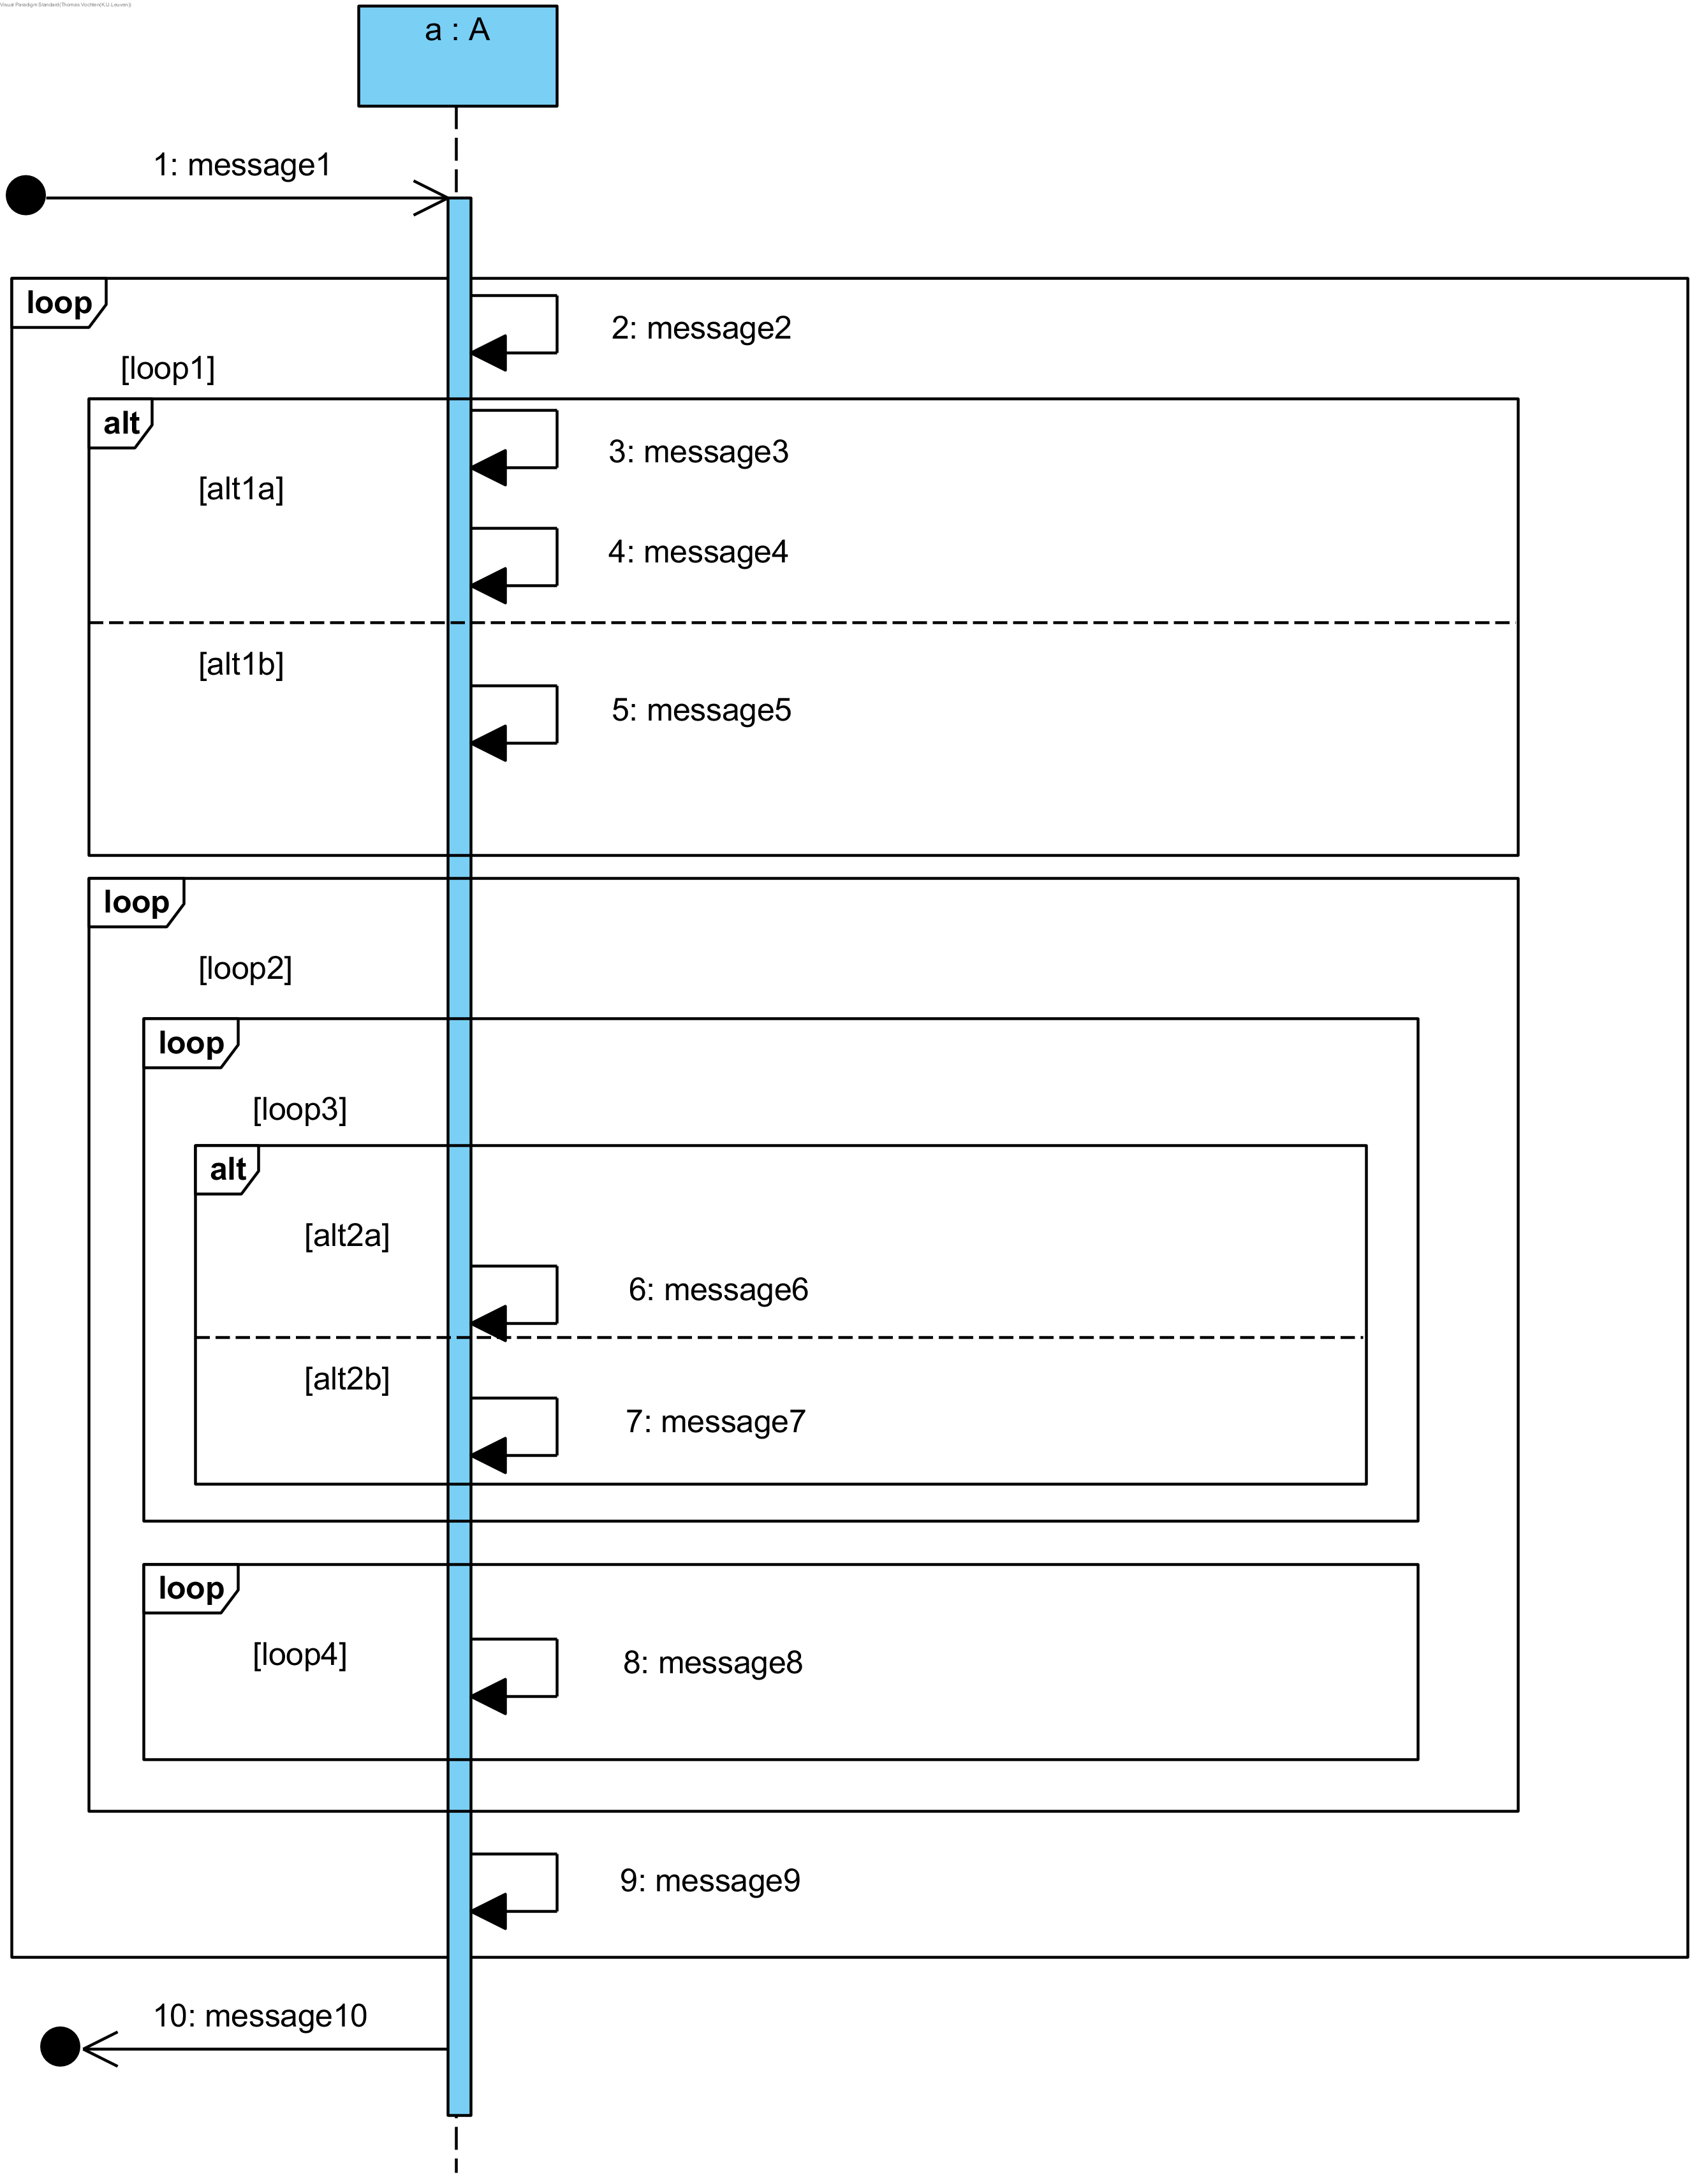
\includegraphics[width=1\textwidth]{chap-gedrag/seq-diagram-frag-ex.png}
	\caption{Sequentiediagram voor een voorbeeldvertaling van combined fragments}
	\label{fig:seq-diagram-frag-ex}
\end{figure}

We gebruiken de voorwaardes van elk respectievelijk fragment om ernaar te verwijzen. \textit{loop1alt1} verwijst naar het alt-fragment als geheel en \textit{loop1alt1if} verwijst naar het \textit{if}-deel.

We roepen algoritme \ref{alg:processCombinedFragment} eerst op op \textit{loop1}. Aangezien het geen ouder heeft en \textit{message1}, wat geen fragment heeft, eraan voorafgaat, noteren we in de uitvoer:

\begin{align*}
	&\transitionentry[message1]{\lnot(loop1)}{message10}
\end{align*}

\todo{definieer wat ik bedoel met deze notatie} In deze context bedoelen we met \textit{loop1} de voorwaarde voor het fragment en niet het fragment zelf.
Er is geen fragment dat v\'o\'or dit fragment komt, dus roepen we algoritme \ref{alg:transition-to-frag} op. \textit{message2} is rechtstreeks deel van \textit{loop1}, dus noteren we in de uitvoer voor dit algoritme:

\begin{align*}
	\transitionentry{loop1}{message2}
\end{align*}

Hierna gaan we verder naar algoritme \ref{alg:wrap-loops} met \textit{loop1alt1} en \textit{loop1loop1} als invoerfragmenten en \textit{allemaal} gezet naar \textbf{true}. \textit{loop1alt1} is geen lusfragment en slaan we over. Vervolgens roepen we algoritme \ref{alg:transition-to-frag} op op \textit{loop1loop1}.
\textit{message6} is niet rechtstreeks deel van \textit{loop1loop1}, dus zetten we \textit{voorwaarde} naar ``\textit{loop1loop1}'' \todo{vraagteken achter voorwaardelabel, maak een commando} en roepen eerst algoritme \ref{alg:transition-to-frag} op op \textit{loop1loop1loop1}. Op dit niveau wordt \textit{voorwaarde} gezet naar ``\textit{loop1loop1} $\land$ \textit{loop1loop1loop1}'' en roepen we algoritme \ref{alg:transition-to-frag} op op \textit{loop1loop1loop1alt}. \textit{message6} en \textit{message7} zijn rechtstreeks deel van \textit{loop1loop1loop1alt}, dus hebben we:

\begin{align*}
	&\transitionentry{loop1loop1 \land loop1loop1loop1 \land loop1loop1loop1alt1if}{message6} \\
	&\transitionentry{loop1loop1 \land loop1loop1loop1 \land loop1loop1loop1alt1then}{message7}
\end{align*}

We keren terug naar het niveau van \textit{loop1loop1}. \textit{loop1loop1loop1} was een lus, dus zetten we \textit{voorwaarde} naar ``\textit{loop1loop} $\land \lnot$ loop1loop1loop1'' en roepen we algoritme \ref{alg:wrap-loops} op op de verzameling met enkel \textit{loop1loop1loop2} als lid. Het resultaat van die oproep is dat we neerschrijven:

\begin{align*}
	\transitionentry{loop1loop1 \land \lnot loop1loop1loop1 \land loop1loop1loop2}{message8}
\end{align*}

We keren terug naar het niveau van \textit{loop1loop1}. Dit fragment heeft verder geen kinderen, dus eindigt deze oproep van algoritme \ref{alg:wrap-loops} hier.

We keren terug naar stap 7 in algoritme \ref{alg:transition-to-frag} voor \textit{loop1}. \textit{loop1alt1} is niet eerder gemarkeerd door algoritme \ref{alg:wrap-loops}, dus roepen we algoritme \ref{alg:transition-to-frag} erop op. Het resultaat van die oproep is:

\begin{align*}
	&\transitionentry{loop1alt1if}{message3} \\
	&\transitionentry{loop1alt1then}{message5}
\end{align*}

Dit markeert het einde van algoritme \ref{alg:transition-to-frag} voor \textit{loop1}. In algoritme \ref{alg:processCombinedFragment} gaan we nu over naar stap 10. Na het uitvoeren van de lus verkrijgen we:

\begin{align*}
	&\transitionentry[message1]{loop1}{message2} \\
	&\transitionentry[message2]{loop1alt1if}{message3} \\
	&\transitionentry[message2]{loop1alt1then}{message5} \\
	&\transitionentry[message4]{loop1loop1 \land loop1loop1loop1 \land loop1loop1loop1alt1if}{message6} \\
	&\transitionentry[message5]{loop1loop1 \land loop1loop1loop1 \land loop1loop1loop1alt1if}{message6} \\
	&\transitionentry[message4]{loop1loop1 \land loop1loop1loop1 \land loop1loop1loop1alt1then}{message7} \\
	&\transitionentry[message5]{loop1loop1 \land loop1loop1loop1 \land loop1loop1loop1alt1then}{message7} \\
	&\transitionentry[message6]{loop1loop1 \land \lnot loop1loop1loop1 \land loop1loop1loop2}{message8} \\
	&\transitionentry[message7]{loop1loop1 \land \lnot loop1loop1loop1 \land loop1loop1loop2}{message8}
\end{align*}

Nu bereiken we stap 18 in algoritme \ref{alg:processCombinedFragment}. Deze stap houdt in dat we algoritme \ref{alg:calcExitForMessages} oproepen op \textit{loop1}.

In stap 1 roepen we eerst algoritme \ref{alg:determineFinalMessage} op op \textit{loop1}. De uitkomst daarvan is dat \textit{message9} herkend wordt als laatste bericht. \textit{loop1} heeft geen ouder, dus gebruiken we algoritme \ref{alg:exitToOutside} met \textit{loop1} en ``$\lnot$ loop1'' als transitievoorwaarde als invoer. Er volgen geen fragmenten op \textit{loop1} en \textit{message10} is geen deel van een fragment, dus noteren we:

\begin{align*}
	\transitionentry{\lnot loop1}{message10}
\end{align*}

Voor stap 6 in algoritme \ref{alg:calcExitForMessages} noteren we:

\begin{align*}
	\transitionentry[message9]{\lnot loop1}{message10}
\end{align*}

Algoritme \ref{alg:calcExitForMessages} gaat nu verder met de kinderen van \textit{loop1}. \textit{loopalt1} komt eerst aan bod, en we bekijken eerst het \textit{if}-deel. Het resultaat van algoritme \ref{alg:determineFinalMessage} is \textit{\{message4, $\epsilon$\}}. \textit{loop1} is de ouder van \textit{loop1alt1} en \textit{message6} is deel van \textit{loop1}, dus we gaan naar stap 11. In wat volgt roepen we algoritme \ref{alg:transition-to-frag} op op \textit{loop1loop1}. Het resultaat daarvan gebruiken we om te noteren:

\begin{align*}
	&\transitionentry[message4]{loop1loop1 \land loop1loop1loop1 \land loop1loop1loop1alt1if}{message6} \\
	&\transitionentry[message4]{loop1loop1 \land loop1loop1loop1 \land loop1loop1loop1alt1then}{message7} \\
	&\transitionentry[message4]{loop1loop1 \land \lnot loop1loop1loop1 \land loop1loop1loop2}{message8}
\end{align*}

Als gevolg van het feit dat \textit{message9} volgt op \textit{loop1loop1}, noteren we ook:

\begin{align*}
	&\transitionentry[message4]{\lnot loop1loop1}{message9}
\end{align*}

Het voorgaande wordt herhaald voor het \textit{else}-deel. Op gelijkaardige wijze voor het \textit{if}-deel leidt dit tot:

\begin{align*}
	&\transitionentry[message5]{loop1loop1 \land loop1loop1loop1 \land loop1loop1loop1alt1if}{message6} \\
	&\transitionentry[message5]{loop1loop1 \land loop1loop1loop1 \land loop1loop1loop1alt1then}{message7} \\
	&\transitionentry[message5]{loop1loop1 \land \lnot loop1loop1loop1 \land loop1loop1loop2}{message8} \\
	&\transitionentry[message5]{\lnot loop1loop1}{message9}
\end{align*}

We gaan terug naar stap 31 voor \textit{loop1}. Algoritme \ref{alg:calcExitForMessages} wordt nu opgeroepen op \textit{loop1loop1}. Via algoritme \ref{alg:determineFinalMessage} concluderen we dat \textit{loop1loop1} geen laatste bericht heeft, dus roepen we algoritme \ref{alg:calcExitForMessages} op op de kinderen. \textit{loop1loop1loop1} komt eerst. Op gelijkaardige wijze gaan we verder naar \textit{loop1loop1loop1alt1}.

Het \textit{if}-deel van \textit{loop1loop1loop1alt1} komt eerst. Algoritme \ref{alg:determineFinalMessage} besluit dat \textit{message6} het laatste bericht is. \textit{message8} is geen deel van \textit{loop1loop1loop1}, dus zetten we \textit{aggregateVoorwaarde} naar ``\textit{$\lnot$ loop1loop1loop1}'' en \textit{fragment} naar \textit{loop1loop1} en gaan naar stap 10. \textit{message8} is deel van \textit{loop1loop1}, dus roepen we algoritme \ref{alg:transition-to-frag} op met \textit{loop1loop1loop2} als argument en concateneren \textit{aggregateVoorwaarde}, wat resulteert in:

\begin{align*}
	\transitionentry[message6]{loop1loop1loop2 \land \lnot loop1loop1loop1}{message8}
\end{align*}

\textit{loop1loop1loop2} is een lus, dus zetten we \textit{fragment} naar \textit{loop1} en gaan naar stap 10. \textit{message8} is deel van \textit{loop1}, maar \textit{loop1loop1} is gemarkeerd in de vorige iteratie en slaan we dus over. We zien wel dat \textit{loop1} een bericht heeft na \textit{message8}, namelijk \textit{message9}, en daarom noteren we:

\begin{align*}
	\transitionentry[message6]{\lnot loop1loop1loop1 \land \lnot loop1loop1loop2 \land \lnot loop1loop1}{message9}
\end{align*}

Met het vinden van dat bericht na \textit{message8}, eindigt het algoritme voor het \textit{if}-deel van \textit{loop1loop1loop1alt1}. Nu komt het \textit{else}-deel van \textit{loop1loop1loop1alt1} aan bod, en gelijkaardig voor het \textit{if}-deel krijgen we:

\begin{align*}
		&\transitionentry[message7]{loop1loop1loop2 \land \lnot loop1loop1loop1}{message8} \\
		&\transitionentry[message7]{\lnot loop1loop1loop1 \land \lnot loop1loop1loop2 \land \lnot loop1loop1}{message9}
\end{align*}

\textit{loop1loop1loop1} is nu volledig behandeld, en we gaan terug naar stap 31 voor \textit{loop1loop1}. We roepen algoritme \ref{alg:calcExitForMessages} op met \textit{loop1loop1loop2} als argument. Algoritme \ref{alg:determineFinalMessage} besluit dat \textit{message8} het laatste bericht is en we zetten \textit{agrregateVoorwaarde} naar ``\textit{$\lnot$ loop1loop1loop2}''. \textit{loop1loop1} heeft geen bericht na \textit{message8}, dus zetten we fragment naar \textit{loop1} en gaan terug naar stap 8. \textit{message9} komt in \textit{loop1} meteen na \textit{message8} en is rechtstreeks deels van \textit{loop1}, dus noteren we:

\begin{align*}
	\transitionentry[message8]{\lnot loop1loop1loop2 \land \lnot loop1loop1}{message9}
\end{align*}

Hier stopt de uitvoering van het algoritme voor \textit{loop1loop1loop2}, en hiermee meteen ook voor \textit{loop1loop1} en \textit{loop1}.

\parbreak

We bereiken stap 19 in algoritme \ref{alg:processCombinedFragment}. In plaats van \textit{loop1} te gebruiken als argument zoals het zou zijn in een echte uitvoering, gebruiken we \textit{loop1loop1loop1alt1} en \textit{loop1loop1loop2} als illustratievere voorbeelden.

De mogelijke laatste berichten van \textit{loop1loop1loop1alt1} zijn \textit{message6} en \textit{message7}. We beschouwen eerst \textit{message6}. \textit{loop1loop1loop1alt1} is geen lusfragment, dus zetten we \textit{fragment} meteen naar \textit{loop1loop1loop1}. \textit{message6} is een laatste bericht daarvan, dus roepen we de variant van algoritme \ref{alg:transition-to-frag} die gebruikt wordt in dit algoritme op met \textit{loop1loop1loop1alt1} als argument. We krijgen als resultaat:

\begin{align*}
	&\transitionentry[message6]{loop1loop1loop1 \land loop1loop1loop1alt1if}{message6} \\
	&\transitionentry[message6]{loop1loop1loop1 \land loop1loop1loop1alt1then}{message7}
\end{align*}

We voegen \textit{loop1loop1loop1} toe aan \textit{uitgesloten} en zetten \textit{aggregateVoorwaarde} naar ``$\lnot loop1loop1loop1$'' en \textit{fragment} naar \textit{loop1loop1}. \textit{message6} is ook een laatste bericht van \textit{loop1loop1}. \textit{loop1loop1loop1} is deel van \textit{uitgesloten} en wordt overgeslagen, maar we zetten \textit{bunderlVoorwaarde} wel naar ``$\lnot loop1loop1loop1$''. \textit{loop1loop1loop2} beschouwen we wel

\section{Interactie tussen meerdere sequentiediagrammen}\label{sec:interaction}
In een project stelt men doorgaans meerdere sequentiediagrammen op die elkaar ook kunnen oproepen. Men gebruikt soms ook recursie in deze diagrammen. In deze sectie beschrijven we hoe we het oproepen van andere sequentiediagrammen en een recursiemechanisme ondersteunen.


	\begin{figure}[h]
		\centering
		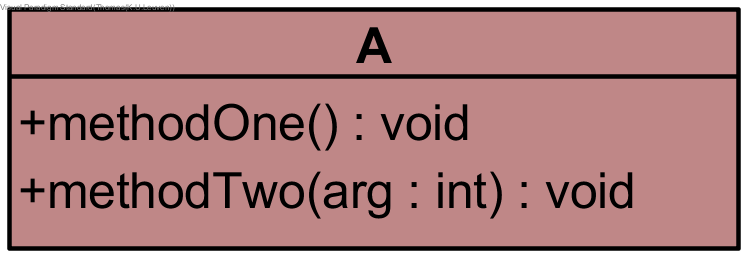
\includegraphics[width=0.25\textwidth]{chap-gedrag/recursion-class.png}
		\caption{Klasse gebruikt in voorbeeld over recursie}
		\label{fig:recursion-class}
	\end{figure}
\begin{landscape}
\thispagestyle{plain}
	\begin{figure}
		\centering
		\begin{subfigure}{\textwidth}
			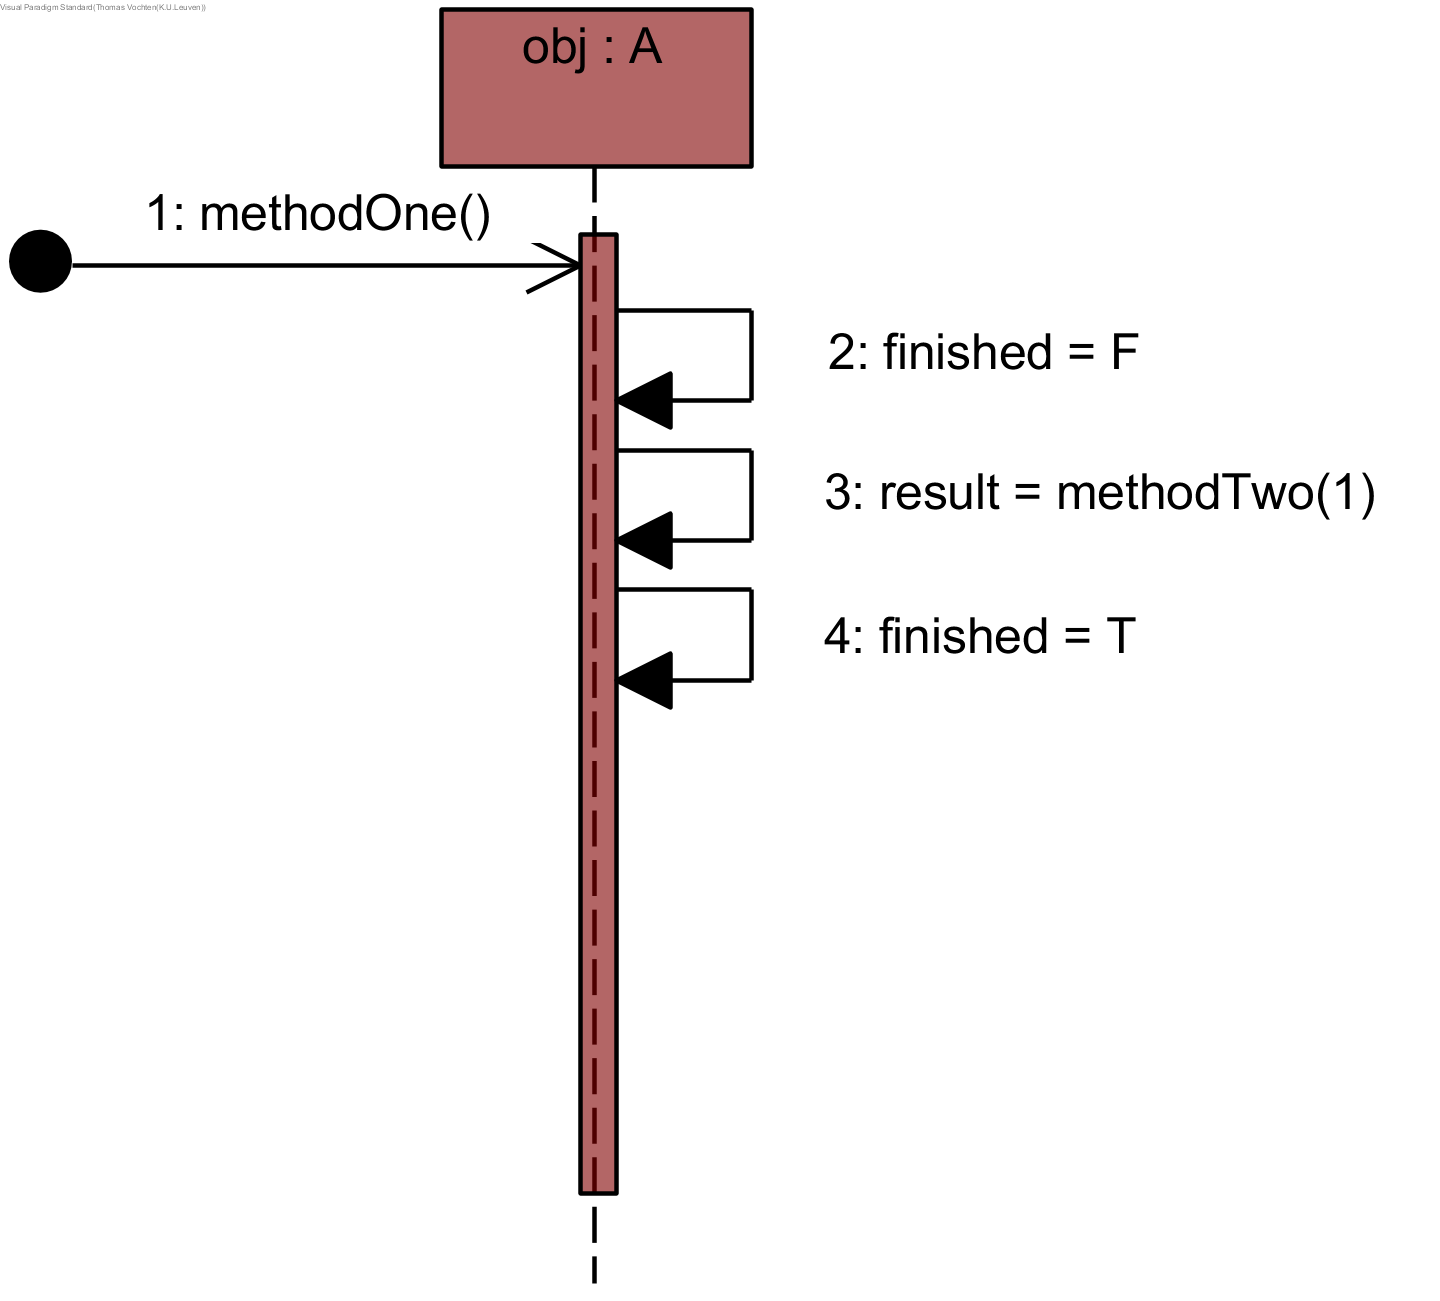
\includegraphics[width=0.4\textwidth]{chap-gedrag/methodOne.png}
			\caption{Sequentiediagram voor methodOne()}
			\label{fig:methodOne}
		\end{subfigure}%
		\begin{subfigure}{\textwidth}
			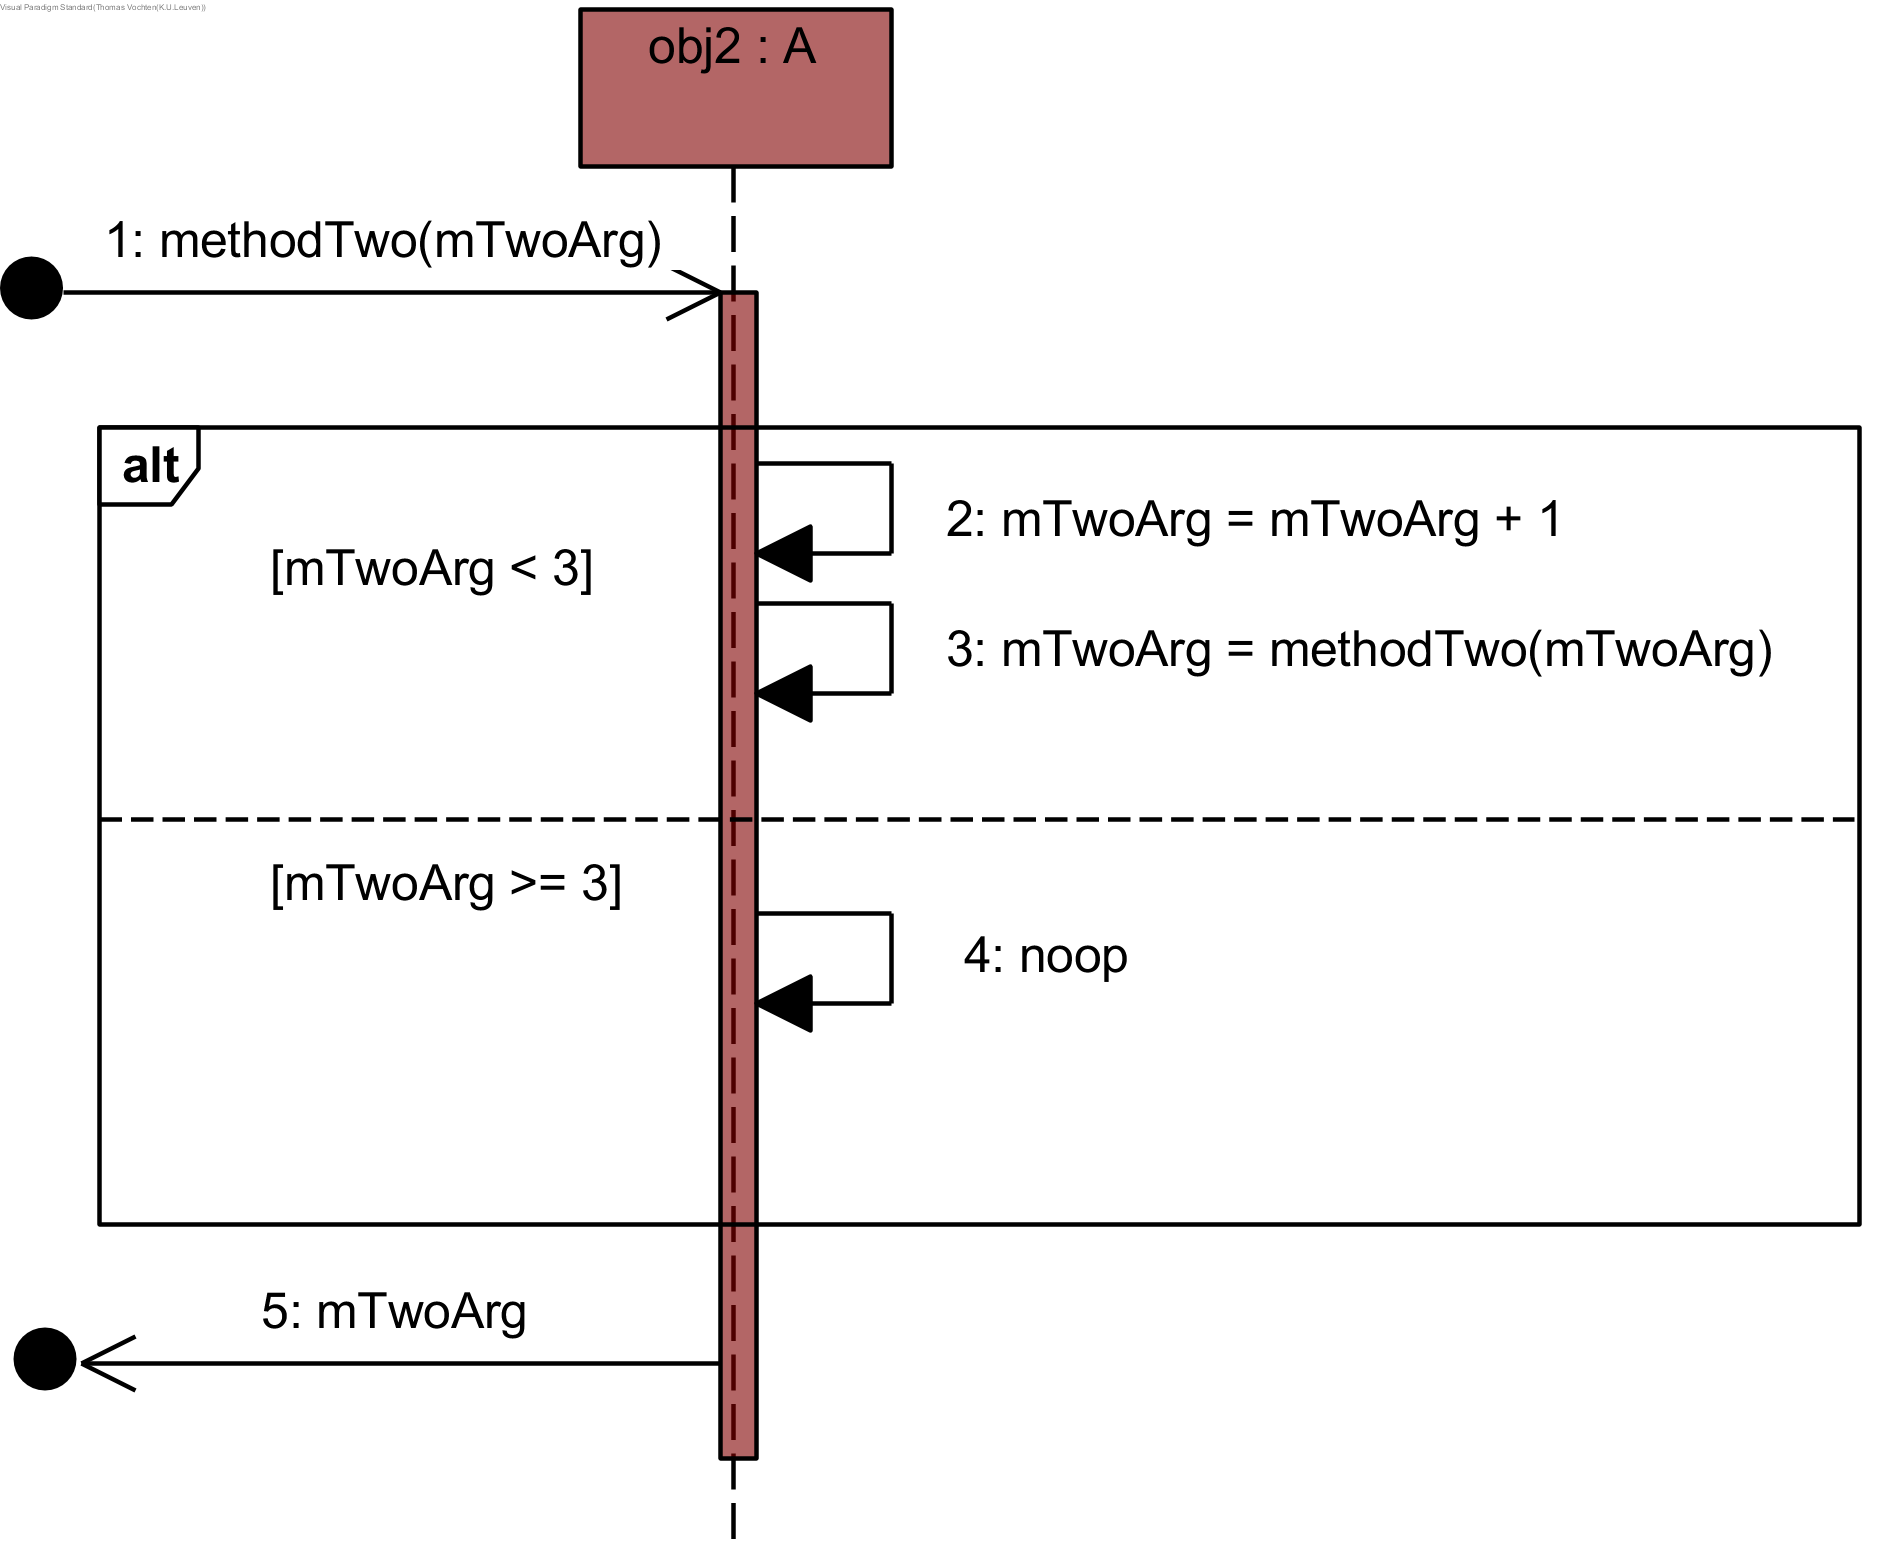
\includegraphics[width=0.75\textwidth]{chap-gedrag/methodTwo.png}
			\caption{Sequentiediagram voor methodTwo()}
			\label{fig:methodtwo}
		\end{subfigure}
		\caption{Sequentiediagrammen voor klasse A in figuur \ref{fig:recursion-class}}
		\label{fig:seq-recursion}
	\end{figure}
\end{landscape}

In de volgende subsecties gebruiken we het voorbeeld uitgebeeld in figuren \ref{fig:recursion-class} en \ref{fig:seq-recursion} om de gebruikte principes te illustreren.

\subsection{Aanpassingen aan \textit{SDPoint}}
Het is niet meer voldoende om \textit{SDPoint}s te modelleren als natuurlijke getallen aangezien elk diagram zijn eigen \textit{SDPoint}s heeft. Om de \textit{SDPoint}s horende bij elk diagram van elkaar te kunnen onderscheiden, maken we van het logisch type \textit{SDPoint} nu een constructed type in IDP. We gebruiken als patroon voor de naamgeving van elk logisch object $<diagramnaam>\_<instructienummer>$. Voor het voorbeeld krijgen we o.a. $methodOne\_2$ en $methodTwo\_3$. We voegen ook een nieuwe functie toe aan het vocabularium dat gegeven een \textit{SDPoint} het volgende \textit{SDPoint} teruggeeft, namelijk $NextSD(SDPoint) : SDPoint$.

Een andere aanpassing is dat we een virtuele \textit{SDPoint} inpassen na elke instructie voor een oproep. Het naamgevingspatroon hiervoor is $<diagramnaam>\_<instructienummer>post$. Aangezien de derde instructie in figuur \ref{fig:methodOne} een oproep is, krijgen we $methodOne\_3post$. Met deze toevoeging ontkoppelen we twee zaken die bij een oproep komen kijken: enerzijds dat het mogelijk is dat het resultaat van een oproep wordt toegekend aan een variabele; en anderzijds dat na een oproep er mogelijks een alt-fragment of lusfragment volgt, en dat het dus v\'o\'or de oproep niet duidelijk is welke de volgende instructie is na de uitvoering van de oproep. Het zou niet mogelijk zijn om deze twee zaken op een correcte manier af te handelen zonder een oproepinstructie op deze manier op te splitsen.

\subsection{Het stapelmechanisme}
Om oproepen van andere sequentiediagrammen correct uit te voeren, moet de theorie bijhouden welke variabelen er bestaan tijdens een bepaalde oproep. Bovendien moet de theorie voor recursieve oproepen ook de waardes van een set variabelen kunnen bewaren v\'o\'or een oproep en die waardes herstellen na een oproep. Hiertoe ontwerpen we een stapelmechanisme. Er gebeuren volgende aanpassingen aan het vocabularium:

\begin{itemize}
	\item Toevoeging van het logisch type $StackLevel \subset \mathbb{N}$: Dit stelt de oproepdiepte van oproep voor.
	\item Toevoeging van een inerti\"ele functie $CurrentStackLevel(Time) : StackLevel$: De oproepdiepte op een bepaald tijdstip.
	\item Toevoeging van een intertieel predicaaat $ReturnPoint(Time, StackLevel, SDPoint)$: Op een bepaald tijdstip, de \textit{SDPoint} naar waar de uitvoering moet terugkeren wanneer de laatste instructie voor de gegeven \textit{StackLevel} bereikt is.
	\item Alle diagramvariabelen worden nu gemodelleerd door een ternair predicaat dat nu ook de oproepdiepte in rekening neemt. Voor het voorbeeld krijgen we dus bijvoorbeeld $FinishedT(Time, StackLevel, bool)$.
\end{itemize}

De volgende subsecties beschrijven hoe we in het definitieblok voor de causatiezinnen dit stapelmechanisme gebruiken.

\subsubsection{Causatiezinnen voor \textit{SDPointAt/2}}\label{sec:sd-rec-cause}
Oproepinstructies betekenen bijkomende uitzonderingen op het normale verloop van \textit{SDPoints} naast deze die voortkomen uit alt-- en lusfragmenten. In dit geval zijn $methodOne\_3$, $methodTwo\_3$, $methodOne\_5$, $methodTwo\_5$ en $finished$ de nieuwe uitzonderingen. $methodOne\_5$ en $methodTwo\_5$ zijn ook \textit{SDPoint}s die niet in het diagram terug te vinden zijn, maar die we zelf toevoegen. Daarmee markeren we het einde van elk van de diagrammen. $finished$ is een speciale \textit{SDPoint} die het einde van de uitvoering aanduidt. De zin die het normale verloop van \textit{SDPoint}s regelt wordt dus:

\begin{align}
	& \nonumber \forall{t}[Time]\forall{s}[SDPoint](C\_SDPointAt(Next(t), NextSD(s) \leftarrow \\ \nonumber &SDPointAt(t,s) \land \lnot((s = methodOne\_3) \lor (s = methodOne\_5) \\ \nonumber &\lor (s = methodTwo\_1) \lor (s = methodTwo\_3) \lor (s = methodTwo\_3post) \\ &\lor (methodTwo\_4) \lor (methodTwo\_5) \lor (s = finished)).
\end{align}

De uitzonderingen als resultaat van een oproep worden als volgt gemodelleerd:

\begin{align}
	 \forall{t}[Time](C\_SDPointAt(Next(t), methodTwo\_1) \leftarrow SDPointAt(t, methodOne\_3).\label{eq:callOne} \\
	 \forall{t}[Time](C\_SDPointAt(Next(t), methodTwo\_1) \leftarrow SDPointAt(t, methodOne\_3).\label{eq:callTwo}
\end{align}

Zin \ref{eq:callOne} resulteert uit instructie 3 van het diagram voor \textit{methodOne} en zin \ref{eq:callTwo} resulteert uit instructie 3 van het diagram voor \textit{methodTwo}.

De tweede aanpassing is dat er een terugkeer moet gebeuren wanneer het einde van een sequentiediagram is bereikt. Hiervoor maken we gebruik van $ReturnPoint/3$:

\begin{align}
	&\nonumber \forall{t}[Time]\forall{s}[SDPoint](C\_SDPointAt(Next(t), s) \leftarrow \\ \nonumber &ReturnPoint(t, CurrentStackLevel(t), s) \land (SDPointAt(t, methodOne\_5) \\ &\lor SDPointAt(t, methodTwo\_5))).\label{eq:sd-return}
\end{align}

Deze zin drukt uit dat het terugkeerpunt dat is genoteerd voor deze oproepdiepte wordt genomen als de volgende \textit{SDPoint} wanneer het einde van een sequentiediagram is bereikt, in dit geval $methodOne\_5$ of $methodTwo\_5$. We schrijven geen nieuwe zin voor $finished$ omdat er niets op volgt.

\subsubsection{Causatiezinnen voor \textit{ReturnPoint/3}}
Wanneer de uitvoering een oproep bereikt, willen we voor de nieuwe oproepdiepte dat het terugkeerpunt wordt gezet naar de \textit{SDPoint} direct na de oproepinstructie. Daarmee krijgen we de volgende twee zinnen:

\begin{align}
	\nonumber &\forall{t}[Time]\forall{st}[StackLevel](C\_ReturnPoint(Next(t), st, methodOne\_3post) \\ &\leftarrow (CurrentStackLevel(t) = (st-1)) \land SDPointAt(t, methodOne\_3)). \\
	\nonumber &\forall{t}[Time]\forall{st}[StackLevel](C\_ReturnPoint(Next(t), st, methodTwo\_3post) \\ &\leftarrow (CurrentStackLevel(t) = (st-1)) \land SDPointAt(t, methodOne\_3)).
\end{align}

We willen ook dat een terugkeerpunt verdwijnt eenmaal dat het wordt gebruikt aan het einde van een diagram. Daarom schrijven we de volgende voorwaarde neer voor het oncausatiepredicaat voor \textit{ReturnPoint/3}:

\begin{align}
 \nonumber &\forall{t}[Time]\forall{st}[StackLevel]\forall{sd}[SDPoint](Cn\_ReturnPoint(Next(t), st, sd) \\ \nonumber &\leftarrow (CurrentStackLevel(t) = st) \land ReturnPoint(t, st, sd) \\ &\land (SDPointAt(t, methodOne\_5) \lor SDPointAt(t, methodTwo\_5))).\label{eq:return-uncauses}
\end{align}

Zinnen \ref{eq:sd-return} en \ref{eq:return-uncauses} samen garanderen dat terugkeerpunten gebruikt worden en verdwijnen wanneer het einde van een diagram is bereikt.

\subsubsection{Causatiezinnen voor \textit{CurrentStackLevel(Time) : StackLevel}}

De oproepdiepte moet toenemen wanneer een oproepinstructie wordt uitgevoerd en afnemen wanneer het einde van een diagram is bereikt. Deze respectievelijke gevallen modelleren we als volgt:

\begin{align}
	\nonumber &\forall{t}[Time]\forall{st}[StackLevel](C\_CurrentStackLevel(Next(t), st) \leftarrow \\ \nonumber &(CurrentStackLevel(t) = (st-1)) \land (SDPointAt(t, methodOne\_3) \\ &\lor SDPointAt(t, methodTwo\_3))). \\
	\nonumber &\forall{t}[Time]\forall{st}[StackLevel](C\_CurrentStackLevel(Next(t), st) \leftarrow \\ \nonumber &(CurrentStackLevel(t) = (st+1)) \land (SDPointAt(t, methodOne\_5) \\ &\lor SDPointAt(t, methodTwo\_5))).
\end{align}

\subsubsection{Causatiezinnen voor oproepobjecten en parameters}
Er komen twee nieuwe soorten variabelen bij: Objecten waarvan een methode wordt opgeroepen en parameters van een methode. In het sequentiediagram voor \textit{methodTwo} is \textit{obj2} de naam van het object dat het eerste bericht ontvangt. Wanneer het diagram voor \textit{methodOne} deze methode oproept, moet \textit{obj2} dus gezet worden naar de juiste waarde, in dit geval \textit{obj} omdat \textit{obj} de methode oproept op zichzelf. Een gelijkaardig geval doet zich voor bij de recursieve oproep in het diagram voor \textit{methodTwo}. Daarom krijgen we de volgende zinnen voor \textit{C\_Obj2T/3}:

\begin{align}
	\nonumber &\forall{t}[Time]\forall{s}[StackLevel]\forall{obj}[A](C\_Obj2T(Next(t), s, obj) \leftarrow
	\\ \nonumber &(CurrentStackLevel(t) = (s-1)) \land SDPointAt(t, methodOne\_3) \\ &\land ObjT(t, (s-1), obj)). \\
	\nonumber &\forall{t}[Time]\forall{s}[StackLevel]\forall{obj}[A](C\_Obj2T(Next(t), s, obj) \leftarrow
	\\ \nonumber &(CurrentStackLevel(t) = (s-1)) \land SDPointAt(t, methodTwo\_3) \\ &\land Obj2T(t, (s-1), obj)).
\end{align}

\textit{mTwoArg} in het diagram voor \textit{methodTwo} is een parameter van \textit{methodTwo} dat ook aangesproken wordt in het diagram zelf. In \textit{methodOne} wordt \textit{mTwoArg} gelijkgesteld aan 1 terwijl in \textit{methodTwo} deze eerst met \'e\'en wordt verhoogd. Daarom krijgen we de drie volgende zinnen:

\begin{align}
	\nonumber &\forall{t}[Time]\forall{s}[StackLevel](C\_MTwoArgT(Next(t), s, 1) \leftarrow \\ &(CurrentStackLevel(t) = (s-1)) \land SDPointAt(t, methodOne\_3)). \\
	\nonumber &\forall{t}[Time]\forall{s}[StackLevel]\forall{n}[int](C\_MTwoArgT(Next(t), s, 1) \leftarrow \\ \nonumber &(CurrentStackLevel(t) = (s-1)) \land SDPointAt(t, methodTwo\_3) \\ &\land MTwoArg(t, (s-1), n)). \\
	\nonumber &\forall{t}[Time]\forall{s}[StackLevel]\forall{n}[int](C\_MTwoArgT(Next(t), s, 1) \leftarrow \\ \nonumber &(CurrentStackLevel(t) = s) \land SDPointAt(t, methodTwo\_2) \\ &\land (\exists{n1}[int](MTwoArg(t, s, n1) \land (n = n1 + 1)))).\label{eq:mtwoarg-inc}
\end{align}

Zin \ref{eq:mtwoarg-inc} demonstreert dat ook buiten oproepinstructies of een terugkeer uit een diagram wordt gekeken naar het oproepniveau. Er wordt immers enkel gekeken of geschreven naar de waarde van de 'versie' van de variabele die overeenkomt met het huidige oproepniveau. Dit komt ook terug bij de variabelen die niet het oproepobject of een parameter van een methode voorstellen.

\subsubsection{Extra veronderstellingen over het ontwerp van sequentiediagrammen}
Om de implementatie van theoriegeneratie zoals beschreven in dit hoofdstuk te vergemakkelijken, zijn er een aantal veronderstellingen ten aanzien van sequentiediagrammen die de gebruiker als invoer geeft. In deze subsectie sommen we deze op:

\begin{itemize}
	\item Er wordt een logisch symbool voorzien voor elke variabele in een sequentiediagram. De naam van dat logisch symbool is gebaseerd op de naam van de variabele, en daarom moeten alle variabelen over alle diagrammen heen een unieke naam hebben. Hoewel de naam van het diagram waarin de variabele voorkomt kan dienen als prefix om de naam van de variabele toch uniek te maken zonder dat tussenkomst van de ontwerper nodig is, hebben we ervoor gekozen om dat niet te doen.
	\item Het type van een variabele kan niet veranderen over instructies heen. Ofwel komt een variabele overeen met een lifeline en wordt het type dus bepaald door de lifeline, ofwel wordt het type bepaald door de instructie die de variabele instantieert.
	\item Een variabele kan geen verzameling voorstellen
	\item Per instructie kan maar \'e\'en associatielink tegelijkertijd genavigeerd worden. Beschouw het voorbeelddiagram van figuur \ref{fig:diagram-voorbeeld}. Als variabele \textit{x} een object van klasse \textit{Item} is, dan zal een oproep van \textit{getInventory()} op \textit{x} een object van klasse \textit{Inventory} opleveren (mocht die associatie zijn ingevuld voor \textit{x}), maar is \textit{getInventory().getCharacter} geen geldige instructie.
	\item Er mogen geen aanpassingen worden aangebracht aan de associatiestructuur voor een model van een klassediagram. Voor een \textit{Character}---\textit{Inventory}-paar geldt bijvoorbeeld dat die verbinding niet verbroken kan worden en dat geen van beide kanten vervangen mag worden door een andere instantie van de respectievelijke klasse. Aangezien associaties van meervoudige multipliciteit als lijsten worden ge\"implementeerd, betekent dit ook dat men geen elementen kan toevoegen aan of verwijderen uit een lijst.
	\item Men kan geen nieuwe objecten instanti\"eren.
	\item Er zijn geen bewerkingen op booleaanse waarden behalve de NOT-functie, die men kan oproepen als \textit{flipBool(boolean)}.
	\item UML legt op dat men voor beide takken van een alt combined fragment de voorwaarde voor de uitvoering die tak moet specificeren. Ook hier wordt verwacht dat de ontwerper dit telkens doet.
	\item Als een diagram een uitvoer heeft, dan mag de instructie die bepaalt welke variabele als uitvoer wordt gebruikt geen onderdeel zijn van een combined fragment.
\end{itemize}

\subsubsection{Uitkomst van de beschreven procedure}
Er zijn geen noemenswaardige veranderingen aan hoe we de toestandszinnen opstellen. Bijlage \ref{app:seq-recursion} bevat de uitkomst van de procedure die we hebben beschreven in deze sectie. 

\section{Extra soorten instructies voor sequentiediagrammen}\label{sec:newlang}
UML is een modelleertaal die wordt gebruikt ter ondersteuning van softwareontwerp in imperatieve programmeertalen. In sequentiediagrammen vertaalt zich dat tot een veelvoud van instructies voor eenvoudige taken zoals het selecteren van het eerste getal verschillend van 0 in een lijst van getallen. Aangezien elke nieuwe instructie in een sequentiediagram leidt tot minstens \'e\'en zin in de gegenereerde theorie, impliceert dit een grote kost in zowel rekentijd als geheugengebruik voor modelexpansie en progressie\"inferentie. Daarom geven we in deze sectie een aanzet tot het integreren van logica in het ontwerp van sequentiediagrammen met het zicht op twee doelen:

\begin{enumerate}
	\item Het totale aantal instructies over alle sequentiediagrammen verminderen
	\item Het aantal tijdstappen die nodig zijn bij modelexpansie of progressie\"inferentie om een bepaalde taak te verrichten verminderen
\end{enumerate}

We houden vast aan de structuur van klasses, associaties, levenslijnen en berichten. Wat volgt is een overzicht van nieuwe soorten instructies die gebruikt kunnen worden in berichten.

\subsection{Nieuwe soorten instructies}

Voorheen kon een variabele maar \'e\'en object of waarde van een primitief type voorstellen. Nu laten we toe dat een variabele een verzameling kan voorstellen. In een sequentiediagram wordt dit voorgesteld als een multi-object zoals in figuur \ref{fig:multi-object}. In de theorie behouden voor namen het patroon $<variabelenaam>T/3$.

We laten op variabelen die een verzameling voorstellen enkele nieuwe instructies toe:

\begin{figure}
	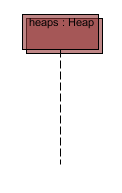
\includegraphics{chap-gedrag/seq-multi-object.png}
	\centering
	\caption{Een multi-object}
	\label{fig:multi-object}
\end{figure}

\begin{itemize}
	\item Voor alle leden van een verzameling tegelijkertijd kan een associatie genavigeerd worden. Als op een verzameling S van objecten van klasse X \textit{getY()} wordt uitgevoerd waar Y de naam is van een klasse geassocieerd met X, dan is het resultaat een verzameling van objecten van klasse Y. Die verzameling bestaat uit alle objecten die in verband staan met minstens \'e\'en object uit S.
	\item $getNumX()$ waar X de naam is van een klasse die in verband staat met de klasse van de verzameling
	\item $EXISTS\ ONE\ WHERE\ [query]$: Geeft \textbf{true} als en slechts als \textit{query} geldt voor minstens \'e\'en lid van de verzameling. \textit{query} betekent hier een instructie die bestaat uit getters van klassevariabelen verbonden met booleaanse connectieven (klassevariabelen kunnen hierbij rechtstreeks vergeleken worden met een getal of string, waar toepasselijk).
	\item $EXISTS\ n\ TO\ m\ WHERE\ [query]$ waar $n \leq m$: Geeft \textbf{true} als en slechts als voor minstens $n$ en ten hoogste $m$ leden van de verzameling geldt dat \textit{query} waar is.
	\item $FOR\ ALL\ APPLIES\ [query]$: Geeft \textbf{true} als en slechts als voor alle leden van de verzameling \textit{query} geldt.
	\item $NOT\ [query]$: geeft \textbf{true} als en slechts als \textit{query} \textbf{false} geeft. \textit{query} kan hier \'e\'en van de voorgaande soorten instructies zijn.
	\item $CHOOSE\ ALL\ WHERE\ APPLIES\ [query]$: Geeft een nieuwe verzameling die bestaat uit alle leden van de originele verzameling waarvoor \textit{query} waar is.
	\item $CHOOSE\ ONE\ WHERE\ APPLIES\ [query]$: Geeft \'e\'en object uit de verzameling waarvoor \textit{query} waar is. Dit vormt een keuzepunt bij simulatie.
	\item $CHOOSE\ n\ TO\ m\ WHERE\ APPLIES\ [query]$ waar $n \leq m$: Geeft een nieuwe verzameling die bestaat uit minstens $n$ en ten hoogste $m$ leden uit de originele verzameling waarvoor \textit{query} waar is. Dit vormt een keuzepunt bij simulatie.
	\item $CHOOSE\ <getalnaam>\ WHERE\ APPLIES\ [query\ dat\ <getalnaam>\ bindt]$: Geeft een nieuwe variabele met als naam \textit{getalnaam} waarvoor geldt dat de waarde voldoet aan \textit{query}. Dit soort instructie kan ook toegepast worden op een variabele dat maar \'e\'en object voorstelt. Dit vormt een keuzepunt bij simulatie.
	\item $SET <klassevariabele> TO <waarde>$: Voor alle leden van de verzameling wordt de waarde van de genoemde klassevariabele veranderd naar de genoemde waarde.
\end{itemize}

We illustreren het gebruik van deze nieuwe instructies door middel van het voorbeeld van figuur \ref{fig:new-nim}, dat een modellering van het bekende spel Nim voorstelt. De beurt gaat eerst aan de gekozen speler. Dan wordt gecontroleerd of alle stapels leeg zijn. Als dat niet het geval is, kiest de speler eerst een stapel en neemt dan minstens \'e\'en object weg van die stapel. Daarna wordt de beurt gegeven aan de volgende speler. Als alle stapels leeg zijn, is de huidige speler de winnaar. Dit stelt dus een versie van Nim voor waar de speler die als laatste een object wegneemt verliest.

\begin{figure}[H]
	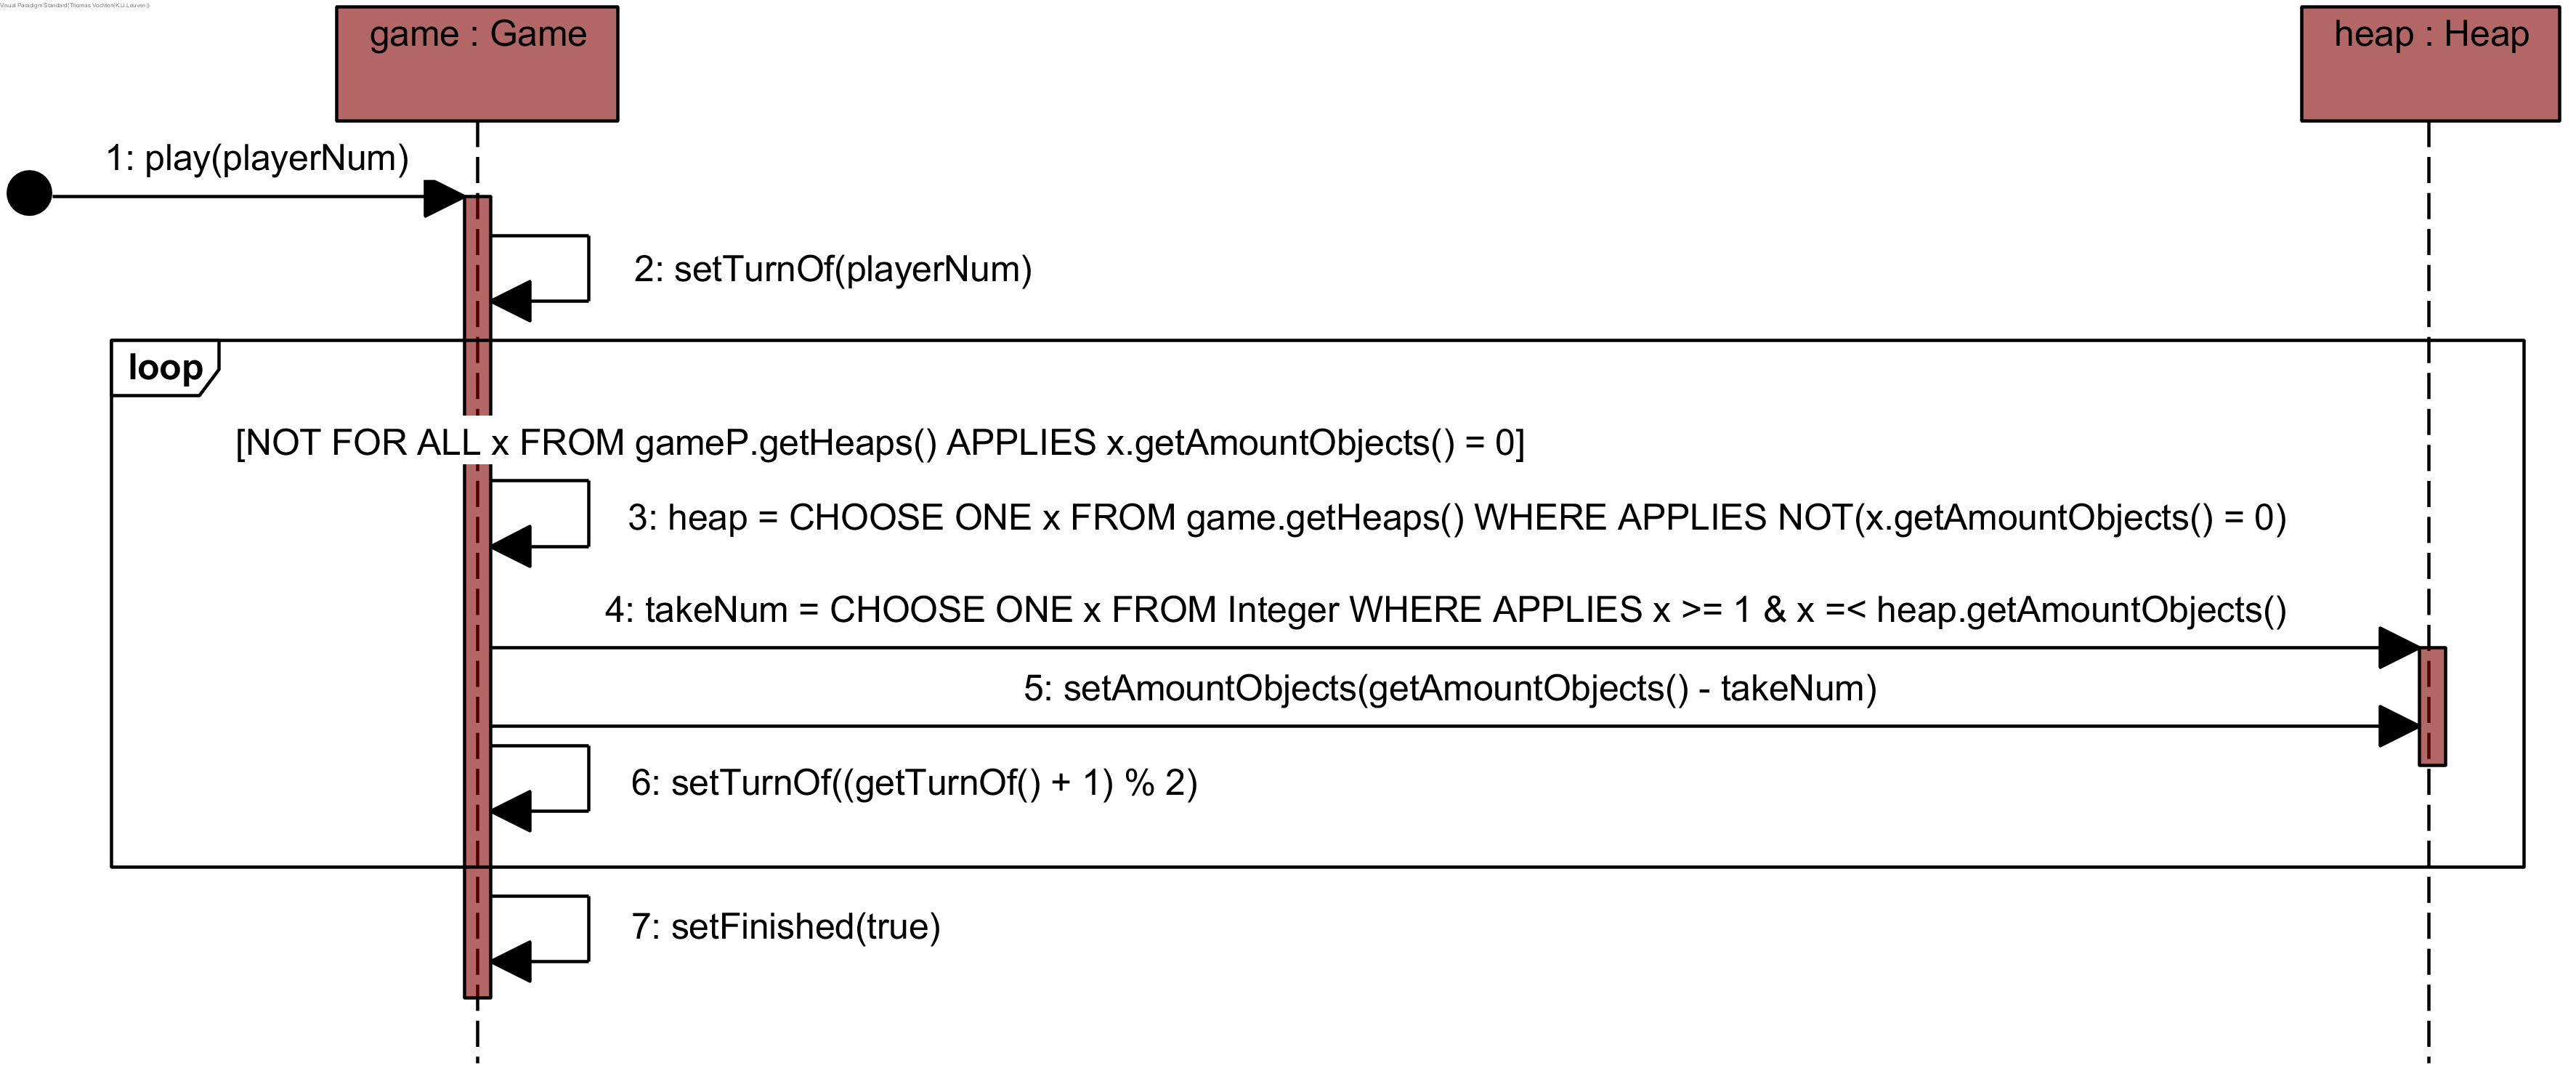
\includegraphics[width=\textwidth]{chap-gedrag/seq-new-nim.png}
	\caption{Een modellering van het spel Nim}
	\label{fig:new-nim}
\end{figure}

De lusvoorwaarde wordt als volgt gebruikt:

\begin{align}
	\nonumber &\forall{t}[Time]\forall{st}[StackLevel](C\_SDPointAt(Next(t), play\_3) \leftarrow \\ \nonumber &(CurrentStackLevel(t) = st) \land (SDPointAt(t, play\_2) \lor SDPointAt(t, play\_6)) \land \\ \nonumber &\lnot{}\exists{g}[Game](GameT(t, st, g) \land{}\forall{h}[Heap](GameandHeap(g, h) \\ &\Rightarrow \exists{n}[LimitedInt](HeapamountObjects(t, h, n) \land n = 0)))). \\
	\nonumber &\forall{t}[Time]\forall{st}[StackLevel](C\_SDPointAt(Next(t), play\_7) \leftarrow \\ \nonumber &(CurrentStackLevel(t) = st) \land SDPointAt(t, play\_6) \land \exists{g}[Game](GameT(t, st, g) \land \\ \nonumber &\forall{h}[Heap](GameandHeap(g, h) \\ &\Rightarrow \exists{n}[LimitedInt](HeapamountObjects(t, h, n) \land n = 0)))).
\end{align}

In instructie 3 wordt de $CHOOSE\ ONE\ WHERE\ APPLIES\ [query]$ instructie gebruikt. We introduceren hier een open predikaat, $ChosenHeap(Time, Heap)$, om ons te helpen deze instructie te vertalen. We voegen de volgende zin toe aan het definitieblok voor diagramvariabelen:

\begin{align}
	\nonumber &\forall{t}[Time]\forall{st}[StackLevel]\forall{h}[Heap](C\_HeapT(Next(t), st, h) \\ &\leftarrow (CurrentStackLevel(t) = st) \land SDPointAt(t, play\_3) \land ChosenHeap(t, h)).
\end{align}

Om ervoor te zorgen dat exact \'e\'en Heap-object wordt gekozen, moeten we voorwaardes leggen op $ChosenHeap/2$. Dit doen we als volgt:

\begin{align}
	&\forall{t}[Time](SDPointAt(t, play\_3) \Rightarrow \exists_{=1}{h}[Heap](ChosenHeap(t, h))). \\
	\nonumber &\forall{t}[Time]\forall{h}[Heap](ChosenHeap(t, h) \Rightarrow (SDPointAt(t, play\_3) \\ \nonumber &\land \exists{g}[Game]\exists{st}[StackLevel]\exists{n}[LimitedInt]((CurrentStackLevel(t) = st) \\ &\land GameT(t, st, g) \land GameandHeap(g, h) \land HeapamountObjects(t, h, n) \land \lnot(n = 0)))).
\end{align}

\todo{meer uitleg bij formules}

Voor instructie 4 introduceren we op een soortgelijke manier een open predikaat $ChosenTake/2$. De zin die we toevoegen aan het definitieblok voor variabelen en de voorwaarden die we opleggen op $ChosenTake/2$ zien er gelijkaardig uit.

Bijlage \ref{code:new-nim} bevat de vertaling van het diagram in figuur \ref{fig:new-nim}.